\documentclass[10pt]{amsart}
%\input{/Dropbox/Math/TexDocument/mysetting.tex}
%\input{mysetting.tex}

\usepackage{amssymb}
\usepackage[leqno]{amsmath}
\usepackage{mathrsfs}
\usepackage{stmaryrd}
\usepackage{chemarrow}
\usepackage[norelsize]{algorithm2e}
\usepackage{enumerate}
\usepackage{graphicx}
\usepackage[pdftex,bookmarksnumbered,bookmarksopen,colorlinks,linkcolor=blue,anchorcolor=black,citecolor=blue,urlcolor=blue]{hyperref}
%\usepackage[dvips,bookmarksnumbered,bookmarksopen,colorlinks,linkcolor=red,anchorcolor=black,citecolor=blue,urlcolor=blue]{hyperref}
\usepackage[all]{xy}
\usepackage{tikz}
\usetikzlibrary{arrows}

\usepackage{multirow}
\usepackage[hyperpageref]{backref}



% comments
%\newcommand{\LC}[1]{\textcolor{cyan}{#1}}
\newcommand{\LC}[1]{\textcolor{red}{#1}}
\newcommand{\XH}[1]{\textcolor{red}{#1}}
%\usepackage[pdftex,colorlinks=true,citecolor=myBlue,linkcolor=myBlue]{hyperref}

  \newcounter{mnote}
  \setcounter{mnote}{0}
  \newcommand{\mnote}[1]{\addtocounter{mnote}{1}
    \ensuremath{{}^{\bullet\arabic{mnote}}}
    \marginpar{\footnotesize\em\color{red}\ensuremath{\bullet\arabic{mnote}}#1}}
  \let\oldmarginpar\marginpar
    \renewcommand\marginpar[1]{\-\oldmarginpar[\raggedleft\footnotesize #1]%
    {\raggedright\footnotesize #1}}

\newtheorem{theorem}{Theorem}[section]
\newtheorem{lemma}[theorem]{Lemma}
\newtheorem{corollary}[theorem]{Corollary}
\newtheorem{proposition}[theorem]{Proposition}
\newtheorem{definition}[theorem]{Definition}
\newtheorem{example}[theorem]{Example}
\newtheorem{exercise}[theorem]{Exercise}
\newtheorem{question}[theorem]{Question}
\newtheorem{remark}[theorem]{Remark}
\newtheorem{alg}[theorem]{Algorithm}

\newcommand{\dx}{\,{\rm d}x}
\newcommand{\dd}{\,{\rm d}}
\newcommand{\bs}{\boldsymbol}
\newcommand{\mcal}{\mathcal}

\DeclareMathOperator*{\img}{img}
%\DeclareMathOperator*{\span}{span}
\newcommand{\curl}{\operatorname{curl}}
\renewcommand{\div}{\operatorname{div}}
%\renewcommand{\grad}{\operatorname{grad}}
\newcommand{\grad}{\operatorname{grad}}
\DeclareMathOperator*{\tr}{tr}
\DeclareMathOperator*{\rot}{rot}
\DeclareMathOperator*{\var}{Var}
\newcommand{\dev}{\operatorname{dev}}
\newcommand{\sym}{\operatorname{sym}}
\newcommand{\skw}{\operatorname{skw}}
\newcommand{\spn}{\operatorname{spn}}
\numberwithin{equation}{section}

\begin{document}
\title[Stabilization-Free VEM]{Stabilization-Free Virtual Element Methods}
\author{Chunyu Chen}%
\address{Hunan Key Laboratory for Computation and Simulation in Science and Engineering; School of Mathematics and Computational Science, Xiangtan University, Xiangtan 411105, P.R.China }%
 \email{202131510114@smail.xtu.edu.cn}%
 \author{Xuehai Huang}%
 \address{School of Mathematics, Shanghai University of Finance and Economics, Shanghai 200433, China}%
 \email{huang.xuehai@sufe.edu.cn}%
\author{Huayi Wei}%
\address{Hunan Key Laboratory for Computation and Simulation in Science and Engineering; School of Mathematics and Computational Science, Xiangtan University, Xiangtan 411105, P.R.China }%
 \email{weihuayi@xtu.edu.cn}%

 \thanks{The second author is the corresponding author. The second author was supported by the National Natural Science Foundation of China Project 12171300, and the Natural Science Foundation of Shanghai 21ZR1480500.}
 \thanks{The first and third authors were supported by NSFC (11871413) and in part by projects
of Education Department of Hunan Provincial of China (19B534, 19A500).}

\makeatletter
\@namedef{subjclassname@2020}{\textup{2020} Mathematics Subject Classification}
\makeatother
\subjclass[2020]{
%65F10;   %% Iterative numerical methods for linear systems
% 58J10;   %%  Differential complexes [See also 35Nxx]; elliptic complexes
65N12;   %%  Stability and convergence of numerical methods for boundary value problems involving PDEs;
% 65N15;   %%  Error bounds for boundary value problems involving PDEs
65N22;   %%  Numerical solution of discretized equations for boundary value problems involving PDEs;
65N30;   %%  Finite element, Rayleigh-Ritz and Galerkin methods for boundary value problems involving PDEs;
%65N55;   %%  Multigrid methods; domain decomposition for boundary value problems involving PDEs;
% 15A69;   %%  Multilinear algebra, tensor calculus
% 15A72;   %%  Vector and tensor algebra, theory of invariants [See also 13A50, 14L24]
}


\begin{abstract}
Stabilization-free virtual element methods in arbitrary degree of polynomial are developed for second order elliptic problems, including a nonconforming virtual element method in arbitrary dimension and a conforming virtual element method in two dimensions.
The key is to construct local $H(\div)$-conforming macro finite element spaces such that the associated $L^2$ projection of the gradient of virtual element functions is computable, and the $L^2$ projector has a uniform lower bound on the gradient of virtual element function spaces in $L^2$ norm.
Optimal error estimates are derived for these stabilization-free virtual element methods.
Numerical results are provided to verify the convergence rates.
\end{abstract}

\keywords{Virtual element, stabilization-Free, macro finite element, norm equivalence, error analysis}


\maketitle

% \tableofcontents

\section{Introduction}

Recently a stabilization-free linear virtual element method, based on a higher order polynomial projection of the gradient of virtual element functions, is devised for Poisson equation in two dimensions in \cite{BerroneBorioMarcon2021,BerroneBorioMarcon2022}, where the degree of polynomial used in projection depends on the number of vertices of the polygon. We refer to~\cite{DAltriMirandaPatrunoSacco2021} for a discussion on similar stabilization-free virtual element methods for plane elasticity problem.
The idea in \cite{BerroneBorioMarcon2021,BerroneBorioMarcon2022} is not easy to extend to construct higher order stabilization-free virtual element methods, and
the analysis is rather elaborate. 
This motivates us to construct stabilization-free virtual element methods in arbitrary degree of polynomial and arbitrary dimension in a unified way.

The key to construct stabilization-free virtual element methods is to find a finite-dimensional space $\mathbb{V}(K)$ and a projector $Q_K$ onto space $\mathbb{V}(K)$ such that
\begin{enumerate}[(C1)]
\item It holds the norm equivalence 
\begin{equation}\label{intro:gradVknormequiv} 
\|Q_{K}\nabla v\|_{0,K}\eqsim \|\nabla v\|_{0,K} \quad \forall~v\in V_k(K)
\end{equation}
on shape function space $V_k(K)$ of virtual elements;
\item The projection $Q_{K}\nabla v$ is computable based on the degrees of freedom (DoFs) of virtual elements for $v\in V_k(K)$.
\end{enumerate}
We can choose $Q_{K}$ as the $L^2$-orthogonal projector with respect to the
inner product $(\cdot, \cdot)_K$. The norm equivalence
\eqref{intro:gradVknormequiv} implies space $\mathbb{V}(K)$ should be
sufficiently large compared with the virtual element space $V_k(K)$.  In
standard virtual element methods, $Q_{k-1}^{K}\nabla v$
\cite{BeiraodaVeigaBrezziMariniRusso2016} or $\nabla\Pi_k^{K}v$
\cite{BeiraoBrezziCangianiManziniEtAl2013,BeiraoBrezziMariniRusso2014,AhmadAlsaediBrezziMariniEtAl2013,AyusodeDiosLipnikovManzini2016}
are used, where $Q_{k-1}^{K}$ is the $L^2$-orthogonal projector onto the
$(k-1)$-th order polynomial space $\mathbb P_{k-1}(K; \mathbb{R}^d)$, and
$\Pi_k^{K}$ is the $H^1$ projection operator onto the $k$-th order polynomial
space $\mathbb P_{k}(K)$.  While only
$$
\|Q_{k-1}^{K}\nabla v\|_{0,K}\lesssim \|\nabla v\|_{0,K}, \quad \|\nabla\Pi_k^{K}v\|_{0,K}\lesssim \|\nabla v\|_{0,K}
$$
hold
rather than the norm equivalence \eqref{intro:gradVknormequiv}, then the additional stabilization term is usually necessary to ensure the coercivity of the discrete bilinear form.
To remove the additional stabilization term, $\mathbb{V}(K)$ is taken as $\mathbb P_{l}(K; \mathbb{R}^d)$ with large enough $l$ even for the lowest order case $k=1$ in \cite{BerroneBorioMarcon2021,BerroneBorioMarcon2022,DAltriMirandaPatrunoSacco2021}, and the virtual element space $V_k(K)$ has to be modified accordingly to make $Q_{l}^{K}\nabla v$ computable.
Instead, we employ $k$-th order or $(k-1)$-th order $H(\div)$-conforming macro finite elements as $\mathbb{V}(K)$ in this paper, and keep the virtual element space $V_k(K)$ as usual ones.


We first construct $H(\div)$-conforming macro finite elements based on a
simplicial partition $\mathcal T_K$ of polytope $K$ in arbitrary dimension. The
shape function space $\mathbb{V}_{k}^{\rm div}(K)$ is a subspace of the $k$th
order Brezzi-Douglas-Marini (BDM) element space on the simplicial partition
$\mathcal T_K$ for $k\geq1$ and the lowest order Raviart-Thomas (RT) element
space for $k=0$, with some constraints. To ensure the $L^2$ projection
$Q_{K,k}^{\div}\nabla v$ onto space $\mathbb{V}_{k}^{\rm div}(K)$ is computable
for virtual element function $v\in V_k(K)$, we require
$\div\boldsymbol{\phi}\in\mathbb P_{\max\{k-1,0\}}(K)$ and
$\boldsymbol{\phi}\cdot\boldsymbol{n}$ on each $(d-1)$-dimensional face of $K$
is a polynomial for $\boldsymbol{\phi}\in\mathbb{V}_{k}^{\rm div}(K)$.  Based on
these considerations and the direct decomposition of an $H(\div)$-conforming
macro finite element space related to $\mathbb{V}_{k}^{\rm div}(K)$, we propose
the unisolvent DoFs for space $\mathbb{V}_{k}^{\rm div}(K)$, and establish the
$L^2$ norm equivalence.  By the way, we use the matrix-vector language to review
a conforming finite element for differential $(d-2)$-form in
\cite{ArnoldFalkWinther2006,Arnold2018}. 




% $$
% \|Q_{K,k-1}^{\div}\nabla v\|_{0,K}\eqsim \|\nabla v\|_{0,K} \quad \forall~v\in V_k(K).
% $$

% $\mathbb{V}_{k-1}^{\rm div}(K)$




By the aid of projector $Q_{K,k}^{\div}$, we advance a stabilization-free nonconforming virtual element method in arbitrary dimension and a stabilization-free conforming virtual element method in two dimensions  for second order elliptic problems.
Indeed, these stabilization-free virtual element methods can be equivalently recast as
primal mixed virtual element methods.
We prove the norm equivalence \eqref{intro:gradVknormequiv} and the well-posedness of these stabilization-free virtual element methods, and derive the optimal error estimates.

The idea on constructing stabilization-free virtual element methods in this paper is simple,
and can be extended to more virtual element methods and more partial differential equations.


The rest of this paper is organized as follows. Notation and mesh conditions are presented in Section~\ref{sec:prelim}. 
In Section~\ref{sec:divmacrofem}, $H(\div)$-conforming macro finite elements in arbitrary dimension are constructed. A stabilization-free nonconforming virtual element method in arbitrary dimension is developed in Section \ref{sec:stabfreencfmvem}. And a stabilization-free conforming virtual element method in two dimensions is devised in Section \ref{sec:stabfreecfmvem}.
Some numerical results are shown in Section \ref{sec:numericalexamps}.


\section{Preliminaries}\label{sec:prelim}

\subsection{Notation}
Let $\Omega\subset \mathbb{R}^d$ be a bounded
polytope. Given a bounded domain $K\subset\mathbb{R}^{d}$ and a
non-negative integer $m$, let $H^m(K)$ be the usual Sobolev space of functions
on $K$.
The corresponding norm and semi-norm are denoted respectively by
$\Vert\cdot\Vert_{m,K}$ and $|\cdot|_{m,K}$. By convention, let $L^2(K)=H^0(K)$. 
Let $(\cdot, \cdot)_K$ be the standard inner product on $L^2(K)$. If $K$ is $\Omega$, we abbreviate
$\Vert\cdot\Vert_{m,K}$, $|\cdot|_{m,K}$ and $(\cdot, \cdot)_K$ by $\Vert\cdot\Vert_{m}$, $|\cdot|_{m}$ and $(\cdot, \cdot)$,
respectively. Let $H_0^m(K)$ be the closure of $\mathcal C_{0}^{\infty}(K)$ with
respect to the norm $\Vert\cdot\Vert_{m,K}$, and $L_0^2(K)$ consist of all functions in $L^2(K)$ with zero mean value.
For integer $k\geq0$,
notation $\mathbb P_k(K)$ stands for the set of all
polynomials over $K$ with the total degree no more than $k$. Set $\mathbb P_{-1}(K)=\{0\}$.
For a banach space $B(K)$, let $B(K; \mathbb{X}):=B(K)\otimes\mathbb{X}$ with $\mathbb{X}=\mathbb{R}^d$ and $\mathbb{K}$, where $\mathbb{K}$ is the set of antisymmetric matrices.
Denote by $Q_k^{K}$ the $L^2$-orthogonal projector onto $\mathbb P_k(K)$ or $\mathbb P_{k}(K; \mathbb{X})$.
For tensor $\boldsymbol{\tau}$, let $\skw\boldsymbol{\tau}:=(\boldsymbol{\tau}-\boldsymbol{\tau}^{\intercal})/2$ be the antisymmetric part of $\boldsymbol{\tau}$.
Denote by $\#S$ the number of elements in a finite set $S$.

For $d$-dimensional polytope $K$, let $\mathcal{F}(K)$ and $\mathcal{E}(K)$ be the set of all $(d-1)$-dimensional faces and $(d-2)$-dimensional faces of $K$ respectively. For $F\in\mathcal{F}(K)$, denote by $\boldsymbol{n}_{K,F}$ be the unit outward normal vector to $\partial K$, which will be abbreviate as $\boldsymbol{n}_F$ or $\boldsymbol{n}$ if not causing any confusion.

For $d$-dimensional simplex $T$,
let $F_i\in\mathcal F(T)$ be the $(d-1)$-dimensional face opposite to vertex $\texttt{v}_i$, $\boldsymbol n_i$ be the unit outward normal to the face $F_i$, and $\lambda_i$ be the barycentric coordinate of $\boldsymbol x$ corresponding to vertex $\texttt{v}_i$, for $i=0, 1, \cdots, d$.
Clearly $\{ \boldsymbol n_1, \boldsymbol n_2, \cdots, \boldsymbol n_d \}$ spans $\mathbb R^d$, and $\{\skw({\boldsymbol n_i\boldsymbol n_j^{\intercal}})\}_{1\leq i<j\leq d}$ spans the antisymmetric space $\mathbb K$. 
For $F\in\mathcal F(T)$, let $\mathcal{E}(F):=\{e\in\mathcal{E}(T): e\subset\partial F\}$.
For $e\in \mathcal E(F)$, denote by $\boldsymbol{n}_{F,e}$ be the unit outward normal vector to $\partial F$.



Let $\{\mathcal {T}_h\}$ denote a family of partitions
of $\Omega$ into nonoverlapping simple polytopes with $h:=\max\limits_{K\in \mathcal {T}_h}h_K$
and $h_K:=\mbox{diam}(K)$.
Denote by $\mathcal F_h^r$ the set of all $(d-r)$-dimensional faces of the partition $\mathcal T_h$ for $r=1,\ldots,d$. Set $\mathcal F_h:=\mathcal F_h^1$ for simplicity. Let $\mathcal F_h^{\partial}$ be the subset of $\mathcal F_h$ including all $(d-1)$-dimensional faces on $\partial\Omega$. 
For any $F\in\mathcal{F}_h$,
let $h_F$ be its diameter and fix a unit normal vector $\boldsymbol{n}_F$.
For a piecewise smooth function $v$, define 
$$
\|v\|_{1,h}^2:=\sum_{K\in\mathcal T_h}\|v\|_{1,K}^2,\quad |v|_{1,h}^2:=\sum_{K\in\mathcal T_h}|v|_{1,K}^2.
$$

For domain $K$, we use $\boldsymbol{H}(\div, K)$ and $\boldsymbol{H}_0(\div, K)$ to denote the standard divergence vector spaces. 
For smooth vector function $\boldsymbol{v}$, let $\nabla\boldsymbol{v}:=(\partial_iv_j)_{1\leq i,j\leq d}$.
On face $F\in\mathcal F_h$, define surface divergence
$$
\div_F\boldsymbol{v}=\div(\boldsymbol{v}-(\boldsymbol{v}\cdot\boldsymbol{n})\boldsymbol{n})=\div\boldsymbol{v}-\partial_n(\boldsymbol{v}\cdot\boldsymbol{n}).
$$
For smooth function $v$, define surface gradient $\nabla_Fv:=\nabla v-(\partial_nv)\boldsymbol{n}$.



\subsection{Mesh conditions}
We impose the following conditions on the mesh $\mathcal T_h$ in this paper:
\begin{itemize}
 \item[(A1)] Each element $K\in \mathcal T_h$ and each face $F\in \mathcal F_h^r$ for $1\leq r\leq d-1$ is star-shaped with a uniformly bounded chunkiness parameter.

 \item[(A2)] There exists a quasi-uniform simplicial mesh $\mathcal T_h^*$ such that each $K\in \mathcal T_h$ is a union of some simplexes in $\mathcal T_h^*$.
\end{itemize}

For $K\in \mathcal T_h$, let $\boldsymbol{x}_K$ be the center of  the largest ball contained in $K$.
Throughout this paper, we use
``$\lesssim\cdots $" to mean that ``$\leq C\cdots$", where
$C$ is a generic positive constant independent of mesh size $h$, but may depend on the chunkiness parameter of the polytope, the degree of polynomials $k$, the dimension of space $d$, and the shape regularity and quasi-uniform constants of the virtual triangulation $\mathcal T^*_h$,
which may take different values at different appearances. And $A\eqsim B$ means $A\lesssim B$ and $B\lesssim A$.

For polytope $K\in \mathcal T_h$, denote by $\mathcal T_K$ the simplicial partition of $K$, which is induced from $\mathcal T_h^*$. Let $\mathcal{F}(\mathcal T_K)$ and $\mathcal{E}(\mathcal T_K)$ be the set of all $(d-1)$-dimensional faces and $(d-2)$-dimensional faces of the simplicial partition $\mathcal T_K$ respectively. Set 
$$
\mathcal{F}^{\partial}(\mathcal T_K):=\{F\in\mathcal{F}(\mathcal T_K): F\subset\partial K\},\quad \mathcal{E}^{\partial}(\mathcal T_K):=\{e\in\mathcal{E}(\mathcal T_K): e\subset\partial K\}.
$$

Hereafter we use $T$ to represent a simplex, and $K$ to denote a general polytope.




\section{$H(\div)$-Conforming Macro Finite Elements}\label{sec:divmacrofem}

In this section we will construct $H(\div)$-conforming macro finite elements in arbitrary dimension.
\subsection{$H(\div)$-conforming finite elements}
For $d$-dimensional polytope $K\in \mathcal T_h$ and $k\geq2$, let 
$$
\boldsymbol{V}_{k-1}^{BDM}(K):=\{\boldsymbol{\phi}\in\bs H(\div, K): \boldsymbol{\phi}|_{T}\in \mathbb P_{k-1}(T;\mathbb R^d) \textrm{ for each } T\in\mathcal T_K\}
$$ 
be the local Brezzi-Douglas-Marini (BDM) element space~\cite{BrezziDouglasMarini1986,BrezziDouglasDuranFortin1987,Nedelec:1986family}, whose degrees of freedom (DoFs) are given by \cite{ChenHuang2021divdiv}
\begin{align}
(\boldsymbol{v}\cdot\boldsymbol{n}, q)_F, & \quad q\in \mathbb P_{k-1}(F), F\in\mathcal F(T), \label{BDMdof1} \\
(\div\boldsymbol{v}, q)_T, & \quad q\in \mathbb P_{k-2}(T)/\mathbb R, \label{BDMdof2} \\
(\boldsymbol{v}, \boldsymbol{q})_T, & \quad \boldsymbol{q}\in \mathbb P_{k-3}(T;\mathbb K)\boldsymbol{x}. \label{BDMdof3}
\end{align}
Define $\mathring{\boldsymbol{V}}_{k-1}^{BDM}(K):=\boldsymbol{V}_{k-1}^{BDM}(K)\cap \boldsymbol{H}_0(\div, K)$.

We also need the lowest order Raviart-Thomas (RT) element space~\cite{BrezziDouglasMarini1986,BrezziDouglasDuranFortin1987,Nedelec:1986family}
$$
\boldsymbol{V}^{RT}(K):=\{\boldsymbol{\phi}\in\bs H(\div, K): \boldsymbol{\phi}|_{T}\in \mathbb P_{0}(T;\mathbb R^d)+\boldsymbol{x}\mathbb P_{0}(T) \textrm{ for each } T\in\mathcal T_K\}.
$$
Define $\mathring{\boldsymbol{V}}^{RT}(K):=\boldsymbol{V}^{RT}(K)\cap \boldsymbol{H}_0(\div, K)$.




\subsection{Finite element for differential $(d-2)$-form}
Now recall the finite element for differential $(d-2)$-form, i.e. $H\Lambda^{d-2}$-conforming finite element in \cite{ArnoldFalkWinther2006,Arnold2018}. We will present the finite element for differential $(d-2)$-form using the proxy of the differential form rather than the differential form itself as in \cite{ArnoldFalkWinther2006,Arnold2018}. 

By Lemma 3.12 in \cite{ChenHuang2021divdiv}, we have the decomposition
\begin{equation}\label{eq:Pkvectordecomp}  
\mathbb P_{k-1}(T;\mathbb R^{d})=\nabla P_k(T)\oplus\mathbb P_{k-2}(T;\mathbb K)\boldsymbol{x}.
\end{equation}

\begin{lemma}\label{lem:skwgrad}
For $\boldsymbol{w}\in\mathbb P_{k-2}(T;\mathbb K)\boldsymbol{x}$ satisfying $(\skw\nabla\boldsymbol{w})\boldsymbol{x}=\boldsymbol{0}$, it holds $\boldsymbol{w}=\boldsymbol{0}$.
\end{lemma}
\begin{proof}
Since
\begin{equation*}%\label{eq:20220224}  
(\skw\nabla\boldsymbol{w})\boldsymbol{x}=\frac{1}{2}(\nabla\boldsymbol{w})\boldsymbol{x}-\frac{1}{2}(\nabla\boldsymbol{w})^{\intercal}\boldsymbol{x}=\frac{1}{2}\nabla(\boldsymbol{w}\cdot\boldsymbol{x})-\frac{1}{2}(I+\boldsymbol{x}\cdot\nabla)\boldsymbol{w},
\end{equation*}
we acquire from $\boldsymbol{w}\cdot\boldsymbol{x}=0$ that $(I+\boldsymbol{x}\cdot\nabla)\boldsymbol{w}=\boldsymbol{0}$, which implies $\boldsymbol{w}=\boldsymbol{0}$.
\end{proof}

\begin{lemma}
The polynomial complex
\begin{equation}\label{eq:polycomplex1}
\mathbb R\xrightarrow{}\mathbb P_k(T)\xrightarrow{\nabla}\mathbb P_{k-1}(T;\mathbb R^d)\xrightarrow{\skw\nabla}\mathbb P_{k-2}(T;\mathbb K)
\end{equation}
is exact.
\end{lemma}
\begin{proof}
Clearly \eqref{eq:polycomplex1} is a complex. It suffices to prove $\mathbb P_{k-1}(T;\mathbb R^d)\cap\ker(\skw\nabla)\subseteq\nabla\mathbb P_{k}(T)$.

For $\boldsymbol{v}\in\mathbb P_{k-1}(T;\mathbb R^d)\cap\ker(\skw\nabla)$, by decomposition \eqref{eq:Pkvectordecomp}, there exist $q\in \mathbb P_k(T)$ and $\boldsymbol{w}\in\mathbb P_{k-2}(T;\mathbb K)\boldsymbol{x}$ such that $\boldsymbol{v}=\nabla q+\boldsymbol{w}$. 
By $\skw\nabla\boldsymbol{v}=\boldsymbol{0}$, we get $\skw\nabla\boldsymbol{w}=\boldsymbol{0}$. 
Apply Lemma~\ref{lem:skwgrad} to derive $\boldsymbol{w}=\boldsymbol{0}$. Thus $\boldsymbol{v}=\nabla q\in\nabla\mathbb P_k(T)$.
\end{proof}

\begin{lemma}
It holds the decomposition
\begin{equation}\label{eq:Pkskwtensordecomp}  
\mathbb P_{k-2}(T;\mathbb K)=\skw\nabla\mathbb P_{k-1}(T;\mathbb R^d)\oplus\big(\mathbb P_{k-2}(T;\mathbb K)\cap\ker(\boldsymbol{x})\big).
\end{equation}
\end{lemma}
\begin{proof}
Thanks to decomposition \eqref{eq:Pkvectordecomp}, we have 
$$
\skw\nabla\mathbb P_{k-1}(T;\mathbb R^d)=\skw\nabla(\mathbb P_{k-2}(T;\mathbb K)\boldsymbol{x}).
$$
By Lemma~\ref{lem:skwgrad}, $\skw\nabla\mathbb P_{k-1}(T;\mathbb R^d)\cap\big(\mathbb P_{k-2}(T;\mathbb K)\cap\ker(\boldsymbol{x})\big)=\{\boldsymbol{0}\}$. Then we only need to check dimensions.
Due to complex \eqref{eq:polycomplex1},
\begin{equation}\label{eq:20220324-1}  
\dim\skw\nabla\mathbb P_{k-1}(T;\mathbb R^d)=\dim\mathbb P_{k-1}(T;\mathbb R^d)-\dim\nabla\mathbb P_k(T).
\end{equation}
On the other side, by space decomposition \eqref{eq:Pkvectordecomp},
$$
\dim\mathbb P_{k-2}(T;\mathbb K)\boldsymbol{x}=\dim\mathbb P_{k-1}(T;\mathbb R^{d})-\dim\nabla\mathbb P_k(T).
$$
Hence $\dim\skw\nabla\mathbb P_{k-1}(T;\mathbb R^d)=\dim\mathbb P_{k-2}(T;\mathbb K)\boldsymbol{x}$, which yields \eqref{eq:Pkskwtensordecomp}.
\end{proof}

% \begin{lemma}
% The polynomial complex
% \begin{equation}\label{eq:polycomplex2}
% \mathbb P_{k-2}(K;\mathbb K)\xrightarrow{\boldsymbol{\tau}\boldsymbol{x}}\mathbb P_{k-1}(K;\mathbb R^d) \xrightarrow{\boldsymbol{v}\cdot\boldsymbol{x}} \mathbb P_k(K)\xrightarrow{\pi_0}\mathbb R
% \end{equation}
% is exact, where $\pi_0q=q(0)$.
% \end{lemma}
% \begin{proof}
% Clearly \eqref{eq:polycomplex2} is a complex, and $\mathbb P_{k-1}(K;\mathbb R^d)\cdot\boldsymbol{x}=\mathbb P_k(K)\cap\ker(\pi_0)$. It suffices to prove $\mathbb P_{k-1}(K;\mathbb R^d)\cap\ker(\cdot\boldsymbol{x})\subseteq\mathbb P_{k-2}(K;\mathbb K)\boldsymbol{x}$.
% \end{proof}

 By \eqref{eq:Pkskwtensordecomp} and \eqref{eq:20220324-1}, it follows
\begin{equation}\label{eq:20220324-2}
\dim\mathbb P_{k-2}(T;\mathbb K)\cap\ker(\boldsymbol{x})=\dim\mathbb P_{k-2}(T;\mathbb K)+\dim\nabla\mathbb P_k(T)- \dim\mathbb P_{k-1}(T;\mathbb R^d).
\end{equation}

With the decomposition \eqref{eq:Pkskwtensordecomp} and $\mathbb P_{k-1}(F;\mathbb R^{d-1})=\nabla_FP_k(F)\oplus\mathbb P_{k-2}(F;\mathbb K)\boldsymbol{x}$, we are ready to define the finite element for differential $(d-2)$-form. Take $\mathbb P_k(T;\mathbb K)$ as the space of shape functions. The degrees of freedom are given by
\begin{align}
((\boldsymbol{n}_1^e)^{\intercal}\boldsymbol{\tau}\boldsymbol{n}_2^e, q)_e, & \quad q\in \mathbb P_k(e), e\in\mathcal E(T), \label{eq:-2formfemdof1} \\
(\div_F(\boldsymbol{\tau}\boldsymbol{n}), q)_F, & \quad q\in \mathbb P_{k-1}(F)/\mathbb R, F\in\mathcal F(T), \label{eq:-2formfemdof21} \\
(\boldsymbol{\tau}\boldsymbol{n}, \boldsymbol{q})_F, & \quad \boldsymbol{q}\in \mathbb P_{k-2}(F;\mathbb K)\boldsymbol{x}, F\in\mathcal F(T), \label{eq:-2formfemdof22} \\
(\div\boldsymbol{\tau}, \boldsymbol{q})_T, & \quad \boldsymbol{q}\in\mathbb P_{k-3}(T;\mathbb K)\boldsymbol{x}, \label{eq:-2formfemdof31} \\
(\boldsymbol{\tau}, \boldsymbol{q})_T, & \quad \boldsymbol{q}\in \mathbb P_{k-2}(T;\mathbb K)\cap\ker(\boldsymbol{x}). \label{eq:-2formfemdof32}
\end{align}
In DoF \eqref{eq:-2formfemdof1}, $\boldsymbol{n}_1^e$ and  $\boldsymbol{n}_2^e$ are two unit normal vectors of $e$ satisfying $\boldsymbol{n}_1^e\cdot\boldsymbol{n}_2^e=0$. 
\begin{lemma}\label{lem:normalskwtensor}
For $e\in\mathcal E(T)$, let $\tilde{\boldsymbol{n}}_1$ and  $\tilde{\boldsymbol{n}}_2$ be another two unit normal vectors of $e$ satisfying $\tilde{\boldsymbol{n}}_1\cdot\tilde{\boldsymbol{n}}_2=0$. Then
$$
\skw(\tilde{\boldsymbol{n}}_1\tilde{\boldsymbol{n}}_2^{\intercal})=\pm\skw(\boldsymbol{n}_1^e(\boldsymbol{n}_2^e)^{\intercal}).
$$
\end{lemma}
\begin{proof}
Notice that there exists an orthonormal matrix $H\in\mathbb R^{2\times2}$ such that 
$(\tilde{\boldsymbol{n}}_1, \tilde{\boldsymbol{n}}_2)=(\boldsymbol{n}_1^e, \boldsymbol{n}_2^e)H$.
Then
\begin{align*}
2\skw(\tilde{\boldsymbol{n}}_1\tilde{\boldsymbol{n}}_2^{\intercal})&=\tilde{\boldsymbol{n}}_1\tilde{\boldsymbol{n}}_2^{\intercal}-\tilde{\boldsymbol{n}}_2\tilde{\boldsymbol{n}}_1^{\intercal}=(\tilde{\boldsymbol{n}}_1, \tilde{\boldsymbol{n}}_2)\begin{pmatrix}
0 & 1 \\
-1 & 0
\end{pmatrix}\begin{pmatrix}
\tilde{\boldsymbol{n}}_1^{\intercal} \\
\tilde{\boldsymbol{n}}_2^{\intercal}  
\end{pmatrix}
\\
&=(\boldsymbol{n}_1^e, \boldsymbol{n}_2^e)H\begin{pmatrix}
0 & 1 \\
-1 & 0
\end{pmatrix}H^{\intercal}(\boldsymbol{n}_1^e, \boldsymbol{n}_2^e)^{\intercal}.
\end{align*}
By direct computation, $H\begin{pmatrix}
0 & 1 \\
-1 & 0
\end{pmatrix}H^{\intercal}={\rm det}(H)\begin{pmatrix}
0 & 1 \\
-1 & 0
\end{pmatrix}$. Hence
$$
2\skw(\tilde{\boldsymbol{n}}_1\tilde{\boldsymbol{n}}_2^{\intercal})=2{\rm det}(H)\skw(\boldsymbol{n}_1^e(\boldsymbol{n}_2^e)^{\intercal}),
$$
which ends the proof.
\end{proof}

\begin{lemma}\label{lem:-2formfemfaceunisolvence}
Let $\boldsymbol{\tau}\in\mathbb P_k(T;\mathbb K)$ and $F\in\mathcal F(T)$.
Assume the degrees of freedom \eqref{eq:-2formfemdof1}-\eqref{eq:-2formfemdof22} on $F$ vanish. 
Then $\boldsymbol{\tau}\boldsymbol{n}|_F=\boldsymbol{0}$.
\end{lemma}
\begin{proof}
Due to \eqref{eq:-2formfemdof1},  we get $(\boldsymbol{n}_1^e)^{\intercal}\boldsymbol{\tau}\boldsymbol{n}_2^e|_e=0$ on each $e\in\mathcal E(F)$, which together with Lemma~\ref{lem:normalskwtensor} indicates $\boldsymbol{n}_{F,e}^{\intercal}\boldsymbol{\tau}\boldsymbol{n}_F|_e=0$. By the unisolvence of BDM element on face $F$, cf. DoFs \eqref{BDMdof1}-\eqref{BDMdof3}, it follows from DoFs \eqref{eq:-2formfemdof21}-\eqref{eq:-2formfemdof22} that $\boldsymbol{\tau}\boldsymbol{n}|_F=\boldsymbol{0}$.
\end{proof}

\begin{lemma}\label{lem:PkKbubblecharac}
For $\boldsymbol{\tau}\in\mathbb P_k(T;\mathbb K)$, $\boldsymbol{\tau}\boldsymbol{n}|_{F_i}=\boldsymbol{0}$ for $i=1,\ldots, d$, if and only if 
\begin{equation}\label{eq:PkKbubblecharac}
\boldsymbol{\tau}=\sum_{1\leq i<j\leq d}\lambda_i\lambda_jq_{ij}\boldsymbol{N}_{ij}
\end{equation}
for some $q_{ij}\in\mathbb P_{k-2}(T)$. Here $\{\boldsymbol{N}_{ij}\}_{1\leq i<j\leq d}$ is the basis of $\mathbb K$ being dual to $\{\skw({\boldsymbol n_i\boldsymbol n_j^{\intercal}})\}_{1\leq i<j\leq d}$, i.e.,
$$
\boldsymbol{N}_{ij}:\skw({\boldsymbol n_l\boldsymbol n_m^{\intercal}})=\delta_{il}\delta_{jm},\quad 1\leq i<j\leq d,\; 1\leq l<m\leq d.
$$
\end{lemma}
\begin{proof}
For $1\leq l\leq d$ but $l\neq i, j$, by the definition of $\boldsymbol{N}_{ij}$, it holds $\boldsymbol{N}_{ij}\boldsymbol{n}_l=\boldsymbol{0}$. Hence for $
\boldsymbol{\tau}=\sum\limits_{1\leq i<j\leq d}\lambda_i\lambda_jq_{ij}\boldsymbol{N}_{ij}
$, obviously we have $\boldsymbol{\tau}\boldsymbol{n}|_{F_i}=\boldsymbol{0}$ for $i=1,\ldots, d$.

On the other side, assume $\boldsymbol{\tau}\boldsymbol{n}|_{F_i}=\boldsymbol{0}$ for $i=1,\ldots, d$. Express $\boldsymbol{\tau}$ as 
$$
\boldsymbol{\tau}=\sum_{1\leq i<j\leq d}p_{ij}\boldsymbol{N}_{ij},
$$
where $p_{ij}=\boldsymbol{n}_i^{\intercal}\boldsymbol{\tau}\boldsymbol{n}_j\in\mathbb P_{k}(T)$.
Therefore $p_{ij}|_{F_i}=p_{ij}|_{F_j}=0$, which ends the proof.
\end{proof}

\begin{lemma}
The degrees of freedom \eqref{eq:-2formfemdof1}-\eqref{eq:-2formfemdof32} are uni-solvent for $\mathbb P_k(T;\mathbb K)$.
\end{lemma}
\begin{proof}
By $\mathbb P_{k-1}(F;\mathbb R^{d-1})=\nabla_FP_k(F)\oplus\mathbb P_{k-2}(F;\mathbb K)\boldsymbol{x}$,
the number of degrees of freedom \eqref{eq:-2formfemdof21}-\eqref{eq:-2formfemdof22} is
$
(d^2+d){k+d-2\choose k-1} - (d+1){k+d-1\choose k}.
$
Using \eqref{eq:Pkvectordecomp} and \eqref{eq:20220324-2},
the number of degrees of freedom \eqref{eq:-2formfemdof1}-\eqref{eq:-2formfemdof32} is
\begin{align*}
&\frac{1}{2}(d^2+d){k+d-2\choose k} + (d^2+d){k+d-2\choose k-1} - (d+1){k+d-1\choose k} \\
&+ \frac{1}{2}(d^2+d){k+d-2\choose k-2}+{k+d\choose k}-(d+1){k+d-1\choose k-1} =\frac{1}{2}(d^2-d){k+d\choose k},
\end{align*}
which equals to $\dim\mathbb P_k(T;\mathbb K)$.

Assume $\boldsymbol{\tau}\in\mathbb P_k(T;\mathbb K)$ and all the degrees of freedom \eqref{eq:-2formfemdof1}-\eqref{eq:-2formfemdof32} vanish. 
It holds from Lemma~\ref{lem:-2formfemfaceunisolvence} that $\boldsymbol{\tau}\boldsymbol{n}|_{\partial T}=\boldsymbol{0}$. Noting that $\boldsymbol{\tau}$ is antisymmetric,  we also have $\boldsymbol{n}^{\intercal}\boldsymbol{\tau}|_{\partial T}=\boldsymbol{0}$. On each $F\in\mathcal F(T)$, it holds
\begin{equation}\label{eq:20220324-3}
\boldsymbol{n}^{\intercal}\div\boldsymbol{\tau}=\div(\boldsymbol{n}^{\intercal}\boldsymbol{\tau})= \div_F(\boldsymbol{n}^{\intercal}\boldsymbol{\tau})+\partial_n(\boldsymbol{n}^{\intercal}\boldsymbol{\tau}\boldsymbol{n})=\div_F(\boldsymbol{n}^{\intercal}\boldsymbol{\tau}).
\end{equation}
Hence $\boldsymbol{n}^{\intercal}\div\boldsymbol{\tau}|_{\partial T}=0$. 
Thanks to DoFs \eqref{BDMdof1}-\eqref{BDMdof3} for BDM element, we acquire from DoF \eqref{eq:-2formfemdof31} and $\div\div\boldsymbol{\tau}=0$ that $\div\boldsymbol{\tau}=\boldsymbol{0}$, which together with DoF \eqref{eq:-2formfemdof32} and decomposition \eqref{eq:Pkskwtensordecomp} gives
$$
(\boldsymbol{\tau}, \boldsymbol{q})_T=0  \quad \forall~\boldsymbol{q}\in \mathbb P_{k-2}(T;\mathbb K).
$$
Applying Lemma~\ref{lem:PkKbubblecharac}, $\boldsymbol{\tau}$ has the expression as in \eqref{eq:PkKbubblecharac}. Taking $\boldsymbol{q}=q_{ij}\skw({\boldsymbol n_i\boldsymbol n_j^{\intercal}})$ in the last equation for $1\leq i<j\leq d$, we get $q_{ij}=0$. Thus $\boldsymbol{\tau}=\boldsymbol{0}$.
\end{proof}


For polygon $K\in \mathcal T_h$, define the local finite element space for differential $(d-2)$-form  
\begin{align*}  
\boldsymbol{V}_{k}^{d-2}(K):=\{\boldsymbol{\tau}\in\bs L^2(K;\mathbb K)&: \boldsymbol{\tau}|_{T}\in \mathbb P_{k}(T;\mathbb K) \textrm{ for each } T\in\mathcal T_K, \\
&\;\;\textrm{ all the DoFs \eqref{eq:-2formfemdof1}-\eqref{eq:-2formfemdof22} are single-valued}\}.
\end{align*}
Thanks to Lemma~\ref{lem:-2formfemfaceunisolvence}, space $\boldsymbol{V}_{k}^{d-2}(K)$ is $H\Lambda^{d-2}$-conforming.
Define $\mathring{\boldsymbol{V}}_{k}^{d-2}(K):=\boldsymbol{V}_{k}^{d-2}(K)\cap \mathring{H}\Lambda^{d-2}(K)$, where $\mathring{H}\Lambda^{d-2}(K)$ is the subspace of $H\Lambda^{d-2}(K)$ with homogeneous boundary condition.
Notice that
 $\boldsymbol{V}_{k}^{d-2}(K)$ is the Lagrange element space for $d=2$,
and $\boldsymbol{V}_{k}^{d-2}(K)$ is the second kind N\'ed\'elec element space for $d=3$ \cite{Nedelec:1986family}. 

% To figure out degrees of freedom for space $\boldsymbol{V}_{k-1}^{\rm div}(K)$,
Recall the local finite element de Rham complexes in \cite{ArnoldFalkWinther2006,Arnold2018}.
For completeness, we will prove the exactness of these complexes.

\begin{lemma}
Let $k\geq2$. Finite element complexes
\begin{equation}\label{eq:localBDMfemderhamcomplex}
\boldsymbol{V}_{k}^{d-2}(K)\xrightarrow{\div\skw}\boldsymbol{V}_{k-1}^{BDM}(K)\xrightarrow{\div} V_{k-2}^{L^2}(K)\to0,    
\end{equation}
\begin{equation}\label{eq:localRTfemderhamcomplex}
\boldsymbol{V}_{1}^{d-2}(K)\xrightarrow{\div\skw}\boldsymbol{V}^{RT}(K)\xrightarrow{\div} V_{0}^{L^2}(K)\to0,    
\end{equation}
\begin{equation}\label{eq:localBDMfemderhamcomplex0}
\mathring{\boldsymbol{V}}_{k}^{d-2}(K)\xrightarrow{\div\skw}\mathring{\boldsymbol{V}}_{k-1}^{BDM}(K)\xrightarrow{\div} \mathring{V}_{k-2}^{L^2}(K)\to0,    
\end{equation}
\begin{equation}\label{eq:localRTfemderhamcomplex0}
\mathring{\boldsymbol{V}}_{1}^{d-2}(K)\xrightarrow{\div\skw}\mathring{\boldsymbol{V}}^{RT}(K)\xrightarrow{\div} \mathring{V}_{0}^{L^2}(K)\to0,    
\end{equation}
are exact, where $\mathring{V}_{k-2}^{L^2}(K):=V_{k-2}^{L^2}(K)/\mathbb R$, and
$$
V_{k-2}^{L^2}(K):=\{v\in L^2(K): v|_{T}\in \mathbb P_{k-2}(T) \textrm{ for each } T\in\mathcal T_K\}.
$$
\end{lemma}
\begin{proof}
We only prove complex \eqref{eq:localBDMfemderhamcomplex}, since the argument for the rest complexes is similar. Clearly \eqref{eq:localBDMfemderhamcomplex} is a complex. We refer to \cite[Section 4]{ChenHuang2021divX} for the proof of $\div\boldsymbol{V}_{k-1}^{BDM}(K)=V_{k-2}^{L^2}(K)$.

Next prove $\boldsymbol{V}_{k-1}^{BDM}(K)\cap\ker(\div)=\div\skw\boldsymbol{V}_{k}^{d-2}(K)$. For $\boldsymbol{v}\in\boldsymbol{V}_{k-1}^{BDM}(K)\cap\ker(\div)$, by Theorem 1.1 in \cite{CostabelMcIntosh2010}, there exists $\boldsymbol{\tau}\in\boldsymbol{H}^1(K;\mathbb K)$ satisfying $\div\boldsymbol{\tau}=\div\skw\boldsymbol{\tau}=\boldsymbol{v}$. Let $\boldsymbol{\sigma}\in \boldsymbol{V}_{k}^{d-2}(K)$ be the nodal interpolation of $\boldsymbol{\tau}$ based on DoFs \eqref{eq:-2formfemdof1}-\eqref{eq:-2formfemdof32}. Thanks to DoF \eqref{eq:-2formfemdof1}, it follows from the integration by parts that
$$
(\div_F(\boldsymbol{\sigma}\boldsymbol{n}), 1)_F=(\boldsymbol{v}\cdot\boldsymbol{n}, 1)_F\quad\forall~F\in\mathcal F(\mathcal T_K),
$$
which together with \eqref{eq:20220324-3} and DoF \eqref{eq:-2formfemdof21} that
$$
(\boldsymbol{n}^{\intercal}\div\boldsymbol{\sigma}, q)_F = (\div_F(\boldsymbol{\sigma}\boldsymbol{n}), q)_F=(\boldsymbol{v}\cdot\boldsymbol{n}, q)_F\quad\forall~q\in \mathbb P_{k-1}(F),F\in\mathcal F(\mathcal T_K).
$$
Therefore, due to DoF \eqref{eq:-2formfemdof31} and the fact $\div\div\boldsymbol{\sigma}=\div\boldsymbol{v}=0$,
we acquire from the unisolvence of DoFs \eqref{BDMdof1}-\eqref{BDMdof3} for BDM element that $\boldsymbol{v}=\div\boldsymbol{\sigma} \in \div\skw\boldsymbol{V}_{k}^{d-2}(K)$.
\end{proof}

Note that $\div\skw=\curl$ for $d=2,3$.
For $k\geq1$, by finite element complexes \eqref{eq:localBDMfemderhamcomplex}-\eqref{eq:localRTfemderhamcomplex0}, we have
\begin{equation}\label{eq:20220324-4}
\dim\div\skw\boldsymbol{V}_{k}^{d-2}(K)-\dim\div\skw\mathring{\boldsymbol{V}}_{k}^{d-2}(K)={k+d-2\choose d-1}\#\mathcal F^{\partial}(\mathcal T_K)-1.
\end{equation}
% \begin{align*}  
% \dim\div\skw\boldsymbol{V}_{k}^{d-2}(K)={k+d-2\choose d-1}\#\mathcal F(\mathcal T_K)+ \left(d{k+d-2\choose d}-{k+d-1\choose d}\right)\#\mathcal T_K, \\
% \dim\div\skw\mathring{\boldsymbol{V}}_{k}^{d-2}(K)={k+d-2\choose d-1}\#\mathcal F^i(\mathcal T_K)+ \left(d{k+d-2\choose d}-{k+d-1\choose d}\right)\#\mathcal T_K+1,
% \end{align*}

\subsection{$H(\div)$-conforming macro finite element}
For each polygon $K\in \mathcal T_h$, 
define shape function space
$$
\boldsymbol{V}_{k-1}^{\rm div}(K):=\{\boldsymbol{\phi}\in\boldsymbol{V}_{k-1}^{BDM}(K): \div\boldsymbol{\phi}\in\mathbb P_{k-2}(K)\},
$$
for $k\geq 2$, and $$
\boldsymbol{V}_{0}^{\rm div}(K):=\{\boldsymbol{\phi}\in\boldsymbol{V}_{0}^{RT}(K): \div\boldsymbol{\phi}\in\mathbb P_{0}(K)\}.
$$
Apparently $\mathbb P_{k-1}(K;\mathbb R^d)\subseteq\boldsymbol{V}_{k-1}^{\rm div}(K)$, $\boldsymbol{V}_{0}^{\rm div}(K)\cap\ker(\div)=\boldsymbol{V}_0^{RT}(K)\cap\ker(\div)$, and $\boldsymbol{V}_{k-1}^{\rm div}(K)\cap\ker(\div)=\boldsymbol{V}_{k-1}^{BDM}(K)\cap\ker(\div)$ for $k\geq2$.


In the following lemma we present a direct sum decomposition of space $\boldsymbol{V}_{k-1}^{\rm div}(K)$.

\begin{lemma}
For $k\geq1$,
it holds
\begin{equation}\label{eq:Vdivlocaldecomp}
\boldsymbol{V}_{k-1}^{\rm div}(K)=\div\skw \boldsymbol{V}_{k}^{d-2}(K) \oplus (\boldsymbol{x}-\boldsymbol{x}_K)\mathbb P_{\max\{k-2,0\}}(K).
\end{equation}
Then the complex
\begin{equation*}
\boldsymbol{V}_{k}^{d-2}(K)\xrightarrow{\div\skw}\boldsymbol{V}_{k-1}^{\rm div}(K)\xrightarrow{\div} \mathbb P_{\max\{k-2,0\}}(K)\to0    
\end{equation*}
is exact.
\end{lemma}
\begin{proof}
We only prove the case $k\geq2$, as the proof for case $k=1$ is similar.
Since $\div:(\boldsymbol{x}-\boldsymbol{x}_K)\mathbb P_{k-2}(K)\to\mathbb P_{k-2}(K)$ is bijective \cite[Lemma 3.1]{ChenHuang2021divdiv}, we have $\div\skw \boldsymbol{V}_{k}^{d-2}(K)\cap(\boldsymbol{x}-\boldsymbol{x}_K)\mathbb P_{k-2}(K)=\{\boldsymbol{0}\}$. Clearly $\div\skw \boldsymbol{V}_{k}^{d-2}(K) \oplus(\boldsymbol{x}-\boldsymbol{x}_K)\mathbb P_{k-2}(K)\subseteq \boldsymbol{V}_{k-1}^{\rm div}(K)$.

On the other side, for $\boldsymbol{\phi}\in \boldsymbol{V}_{k-1}^{\rm div}(K)$, by $\div\boldsymbol{\phi}\in \mathbb P_{k-2}(K)$, there exists a $q\in\mathbb P_{k-2}(K)$ such that $\div((\boldsymbol{x}-\boldsymbol{x}_K)q)=\div\boldsymbol{\phi}$, i.e. $\boldsymbol{\phi}-(\boldsymbol{x}-\boldsymbol{x}_K)q\in\boldsymbol{V}_{k-1}^{\rm div}(K)\cap\ker(\div)=\boldsymbol{V}_{k-1}^{BDM}(K)\cap\ker(\div)$. Thanks to finite element complex \eqref{eq:localBDMfemderhamcomplex}, $\boldsymbol{\phi}-(\boldsymbol{x}-\boldsymbol{x}_K)q\in\div\skw \boldsymbol{V}_{k}^{d-2}(K)$. Thus \eqref{eq:Vdivlocaldecomp} follows.
\end{proof}

Based on the space decomposition \eqref{eq:Vdivlocaldecomp} and the degrees of freedom of BDM element, we propose the following DoFs for space $\boldsymbol{V}_{k-1}^{\rm div}(K)$
\begin{align}
    (\boldsymbol{\phi}\cdot\boldsymbol{n}, q)_F & \quad\forall~q\in\mathbb P_{k-1}(F) \textrm{ on each }  F\in\mathcal F^{\partial}(\mathcal T_K), \label{Vdivdof1}\\
    (\div\boldsymbol{\phi}, q)_K & \quad\forall~q\in\mathbb P_{\max\{k-2,0\}}(K)/\mathbb R, \label{Vdivdof2} \\
    (\boldsymbol{\phi}, \bs q)_K & \quad\forall~\bs q\in \div\skw\mathring{\boldsymbol{V}}_{k}^{d-2}(K)=\div\mathring{\boldsymbol{V}}_{k}^{d-2}(K). \label{Vdivdof3}
\end{align}
% where $\mathring{\boldsymbol{V}}_{k-1}^{\rm div}(K):=\boldsymbol{V}_{k-1}^{\rm div}(K)\cap\boldsymbol{H}_0(\div, K)$.
% where $\mathcal E^{\partial}(\mathcal T_K):=\{e\in\mathcal E(\mathcal T_K): e\subset\partial K\}$.
% DoF \eqref{Vdivdof3} will disappear when $\mathcal T_K=\{K\}$ is a simplex.
\begin{lemma}
The set of DoFs \eqref{Vdivdof1}-\eqref{Vdivdof3} is uni-solvent for space $\boldsymbol{V}_{k-1}^{\rm div}(K)$.
\end{lemma}
\begin{proof}
By \eqref{eq:20220324-4} and \eqref{eq:Vdivlocaldecomp},
the number of DoFs \eqref{Vdivdof1}-\eqref{Vdivdof3} is
\begin{align*}
&\quad {k+d-2\choose d-1}\#\mathcal F^{\partial}(\mathcal T_K)+\dim\mathbb P_{\max\{k-2,0\}}(K)-1+\dim\div\skw\mathring{\boldsymbol{V}}_{k}^{d-2}(K) \\
&=\dim\div\skw\boldsymbol{V}_{k}^{d-2}(K)+\dim\mathbb P_{\max\{k-2,0\}}(K)=\dim\boldsymbol{V}_{k-1}^{\rm div}(K).
\end{align*}
% By \eqref{eq:Vdivlocaldecomp},
% the number of DoFs \eqref{Vdivdof1}-\eqref{Vdivdof3} equals to $\dim\boldsymbol{V}_{k-1}^{\rm div}(K)$.

Assume $\boldsymbol{\phi}\in\boldsymbol{V}_{k-1}^{\rm div}(K)$ and all the DoFs \eqref{Vdivdof1}-\eqref{Vdivdof3} vanish. By the vanishing DoF~\eqref{Vdivdof1}, $\boldsymbol{\phi}\in \boldsymbol{H}_0(\div, K)$ and $\div\boldsymbol{\phi}\in L_0^2(K)$. Then it follows from the vanishing DoF~\eqref{Vdivdof2} that $\div\boldsymbol{\phi}=0$. 
Thanks to the exactness of complexes \eqref{eq:localBDMfemderhamcomplex0}-\eqref{eq:localRTfemderhamcomplex0}, $\boldsymbol{\phi}\in\div\skw\mathring{\boldsymbol{V}}_{k}^{d-2}(K)$. Therefore $\boldsymbol{\phi}=\boldsymbol{0}$ holds from the vanishing DoF~\eqref{Vdivdof3}.
\end{proof}



\begin{remark}\rm
When $K$ is a simplex and $\mathcal T_K=\{K\}$, thanks to DoF \eqref{BDMdof3} for the BDM element, DoF \eqref{Vdivdof3} can be replaced by 
$$
(\boldsymbol{\phi}, \bs q)_K \quad\forall~\bs q\in \mathbb P_{k-3}(K;\mathbb K)\boldsymbol{x}
$$
for $k\geq3$.
And DoF \eqref{Vdivdof3} disappears for $k=1$ and $k=2$.
\end{remark}

% \begin{lemma}
% For $p\in V_{1}^{\grad}(K)$, it holds
% \begin{equation}\label{eq:V1gradKprop}
% \|\curl p\|_{0,K}\lesssim \sup_{w\in\mathring{V}_{1}^{\grad}(K)}\frac{(\curl p, \curl w)_K}{\|\curl w\|_{0,K}} +\sum_{e\in\mathcal E^{\partial}(\mathcal T_K)}h_e^{1/2}\|(\curl p)\cdot\boldsymbol{n}\|_{0,e}.
% \end{equation}
% \end{lemma}
% \begin{proof}
% Take a vertex $\delta_0\in\mathcal V^{\partial}(\mathcal T_K)$. Without loss of generality, assume $p(\delta_0)=0$. Let $\tilde p\in V_{1}^{\grad}(K)$ satisfy $\tilde p|_{\partial K}=p|_{\partial K}$ and $\tilde p(\delta)=0$ for all $\delta\in\mathcal V^{i}(\mathcal T_K)$. Then $p-\tilde p\in\mathring{V}_{1}^{\grad}(K)$, and
% \begin{align*}
% \|\curl (p-\tilde p)\|_{0,K}&= \sup_{w\in\mathring{V}_{1}^{\grad}(K)}\frac{(\curl(p-\tilde p), \curl w)_K}{\|\curl w\|_{0,K}} \\
% &\lesssim \|\curl\tilde p\|_{0,K}+\sup_{w\in\mathring{V}_{1}^{\grad}(K)}\frac{(\curl p, \curl w)_K}{\|\curl w\|_{0,K}}.
% \end{align*}
% By the triangle inequality, the last inequality implies
% \begin{equation}\label{eq:20220203}
% \|\curl p\|_{0,K}\lesssim \|\curl\tilde p\|_{0,K}+\sup_{w\in\mathring{V}_{1}^{\grad}(K)}\frac{(\curl p, \curl w)_K}{\|\curl w\|_{0,K}}.
% \end{equation}

% On the other side, applying the inverse inequality and the scaling argument,
% \begin{align*}
% \|\curl\tilde p\|_{0,K}^2&\lesssim \sum_{\tau\in\mathcal T_K}h_{\tau}^{-2}\|\tilde p\|_{0,\tau}^2\eqsim \sum_{\delta\in\mathcal V^{\partial}(\mathcal T_K)} \tilde p^2(\delta)=\sum_{\delta\in\mathcal V^{\partial}(\mathcal T_K)} (p(\delta)-p(\delta_0))^2 \\
% &\lesssim \sum_{e\in\mathcal E^{\partial}(\mathcal T_K)}h_e\|(\curl p)\cdot\boldsymbol{n}\|_{0,e}^2.
% \end{align*}
% Therefore \eqref{eq:V1gradKprop} follows from \eqref{eq:20220203} and the last inequality.
% \end{proof}

Next we consider the norm equivalence of space $\boldsymbol{V}_{k-1}^{\rm div}(K)$.


\begin{lemma}\label{lem:Vkm1divnormequivalence}
For $\boldsymbol{\phi}\in\boldsymbol{V}_{k-1}^{\rm div}(K)$, it holds the norm equivalence
\begin{equation}\label{eq:Vkm1divnormequivalence}
\|\boldsymbol{\phi}\|_{0,K}\eqsim h_K\|\div\boldsymbol{\phi}\|_{0,K} + \sup_{\boldsymbol{\psi}\in\div\mathring{\boldsymbol{V}}_{k}^{d-2}(K)}\frac{(\boldsymbol{\phi}, \boldsymbol{\psi})_K}{\|\boldsymbol{\psi}\|_{0,K}} +\sum_{F\in\mathcal F^{\partial}(\mathcal T_K)}h_F^{1/2}\|\boldsymbol{\phi}\cdot\boldsymbol{n}\|_{0,F}.
\end{equation}
\end{lemma}
\begin{proof}
By the inverse inequality \cite[Lemma 10]{Huang2020} and the trace inequality \cite[(2.18)]{BrennerSung2018}, we have
\begin{align*}
&\quad h_K\|\div\boldsymbol{\phi}\|_{0,K}+\sup_{\boldsymbol{\psi}\in\div\mathring{\boldsymbol{V}}_{k}^{d-2}(K)}\frac{(\boldsymbol{\phi}, \boldsymbol{\psi})_K}{\|\boldsymbol{\psi}\|_{0,K}} +\sum_{F\in\mathcal F^{\partial}(\mathcal T_K)}h_F^{1/2}\|\boldsymbol{\phi}\cdot\boldsymbol{n}\|_{0,F}\\
&\lesssim \|\div\boldsymbol{\phi}\|_{-1,K} + \|\boldsymbol{\phi}\|_{0,K} \lesssim \|\boldsymbol{\phi}\|_{0,K}.    
\end{align*}

Next we focus on the proof of the other side. Again we only prove the case $k\geq2$, whose argument can be applied to case $k=1$. Take $\boldsymbol{\phi}_1\in\boldsymbol{V}_{k-1}^{BDM}(K)$ such that $\boldsymbol{\phi}_1\cdot\boldsymbol{n}|_{\partial K}=\boldsymbol{\phi}\cdot\boldsymbol{n}_{\partial K}$, and all the DoFs \eqref{BDMdof1}-\eqref{BDMdof3} of $\boldsymbol{\phi}_1$ in the interior of $K$ vanish. We have
\begin{equation}\label{eq:20220324-5}
\|\boldsymbol{\phi}_1\|_{0,K}\eqsim \sum_{F\in\mathcal F^{\partial}(\mathcal T_K)}h_F^{1/2}\|\boldsymbol{\phi}\cdot\boldsymbol{n}\|_{0,F},
\end{equation}
$$
\|\div\boldsymbol{\phi}_1\|_{0,T}^2=\|Q_0^T(\div\boldsymbol{\phi}_1)\|_{0,T}^2
\leq\frac{1}{|T|}\sum_{F\in\mathcal F(T)\cap\mathcal F^{\partial}(\mathcal T_K)}|F|\|\boldsymbol{\phi}\cdot\boldsymbol{n}\|_{0,F}^2\quad\forall~T\in\mathcal T_K.
$$
Then let $w\in H^1(K)/\mathbb R$ be the solution of 
$$
\begin{cases}
-\Delta w= \div(\boldsymbol{\phi}-\boldsymbol{\phi}_1)\quad\textrm{ in } K, \\
\;\;\partial_nw=0\qquad\qquad\quad\;\;\,\textrm{ on } \partial K.
\end{cases}
$$
The weak formulation is
$$
(\nabla w, \nabla v)_K=(\div(\boldsymbol{\phi}-\boldsymbol{\phi}_1), v)_K\quad\forall~v\in H^1(K)/\mathbb R.
$$
Obviously we have
$$
\|\nabla w\|_{0,K}\lesssim h_K\|\div(\boldsymbol{\phi}-\boldsymbol{\phi}_1)\|_{0,K}\lesssim h_K\|\div\boldsymbol{\phi}\|_{0,K} +\sum_{F\in\mathcal F^{\partial}(\mathcal T_K)}h_F^{1/2}\|\boldsymbol{\phi}\cdot\boldsymbol{n}\|_{0,F}.
$$
Let $I_K^{\div}: \boldsymbol{H}_0(\div,K)\to\mathring{\boldsymbol{V}}_{k-1}^{BDM}(K)$ be the $L^2$-bounded commuting projection operator in \cite{ChristiansenWinther2008}. Set $\boldsymbol{\phi}_2=-I_K^{\div}(\nabla w)\in\mathring{\boldsymbol{V}}_{k-1}^{BDM}(K)$. We have
\begin{equation}\label{eq:20220324-6}
\div\boldsymbol{\phi}_2=-\Delta w=\div(\boldsymbol{\phi}-\boldsymbol{\phi}_1),
\end{equation}
\begin{equation}\label{eq:20220324-7}
\|\boldsymbol{\phi}_2\|_{0,K}\lesssim \|\nabla w\|_{0,K}\lesssim h_K\|\div\boldsymbol{\phi}\|_{0,K} +\sum_{F\in\mathcal F^{\partial}(\mathcal T_K)}h_F^{1/2}\|\boldsymbol{\phi}\cdot\boldsymbol{n}\|_{0,F}.
\end{equation}
By \eqref{eq:20220324-6}, $\boldsymbol{\phi}-\boldsymbol{\phi}_1-\boldsymbol{\phi}_2\in\mathring{\boldsymbol{V}}_{k-1}^{BDM}(K)\cap\ker(\div)$, which together the exactness of complex \eqref{eq:localBDMfemderhamcomplex0} indicates $\boldsymbol{\phi}-\boldsymbol{\phi}_1-\boldsymbol{\phi}_2\in\div\mathring{\boldsymbol{V}}_{k}^{d-2}(K)$. Hence
\begin{align*}  
\|\boldsymbol{\phi}\|_{0,K}&\lesssim \|\boldsymbol{\phi}_1\|_{0,K}+\|\boldsymbol{\phi}_2\|_{0,K}+\|\boldsymbol{\phi}-\boldsymbol{\phi}_1-\boldsymbol{\phi}_2\|_{0,K} \\
&\lesssim \|\boldsymbol{\phi}_1\|_{0,K}+\|\boldsymbol{\phi}_2\|_{0,K}+\sup_{\boldsymbol{\psi}\in\div\mathring{\boldsymbol{V}}_{k}^{d-2}(K)}\frac{(\boldsymbol{\phi}-\boldsymbol{\phi}_1-\boldsymbol{\phi}_2, \boldsymbol{\psi})_K}{\|\boldsymbol{\psi}\|_{0,K}} \\
&\lesssim \|\boldsymbol{\phi}_1\|_{0,K}+\|\boldsymbol{\phi}_2\|_{0,K}+\sup_{\boldsymbol{\psi}\in\div\mathring{\boldsymbol{V}}_{k}^{d-2}(K)}\frac{(\boldsymbol{\phi}, \boldsymbol{\psi})_K}{\|\boldsymbol{\psi}\|_{0,K}}.
\end{align*}
Finally \eqref{eq:Vkm1divnormequivalence} holds from \eqref{eq:20220324-5} and \eqref{eq:20220324-7}.
\end{proof}


Let 
$$
\mathbb{V}_{k-1}^{\rm div}(K):=\{\boldsymbol{\phi}\in\boldsymbol{V}_{k-1}^{\rm div}(K): \boldsymbol{\phi}\cdot\boldsymbol{n}|_F\in\mathbb P_{k-1}(F) \quad\forall~F\in\mathcal F(K)\}.
$$
Due to DoFs \eqref{Vpdivdof1}-\eqref{Vpdivdof3} for $\boldsymbol{V}_{k-1}^{\rm div}(K)$, a set of unisolvent DoFs for $\mathbb{V}_{k-1}^{\rm div}(K)$ is 
\begin{align}
    (\boldsymbol{\phi}\cdot\boldsymbol{n}, q)_F & \quad\forall~q\in\mathbb P_{k-1}(F) \textrm{ on each }  F\in\mathcal F(K), \label{Vpdivdof1}\\
    (\div\boldsymbol{\phi}, q)_K & \quad\forall~q\in\mathbb P_{\max\{k-2,0\}}(K)/\mathbb R, \label{Vpdivdof2} \\
    (\boldsymbol{\phi}, \bs q)_K & \quad\forall~\bs q\in \div\mathring{\boldsymbol{V}}_{k}^{d-2}(K). \label{Vpdivdof3}
\end{align}

As an immediate result of Lemma~\ref{lem:Vkm1divnormequivalence}, we get the following norm equivalence of space $\mathbb{V}_{k-1}^{\rm div}(K)$.
\begin{corollary}
For $\boldsymbol{\phi}\in\mathbb{V}_{k-1}^{\rm div}(K)$, it holds the norm equivalence
\begin{equation}\label{eq:Vkm1divnormequiv}
\|\boldsymbol{\phi}\|_{0,K}\eqsim h_K\|\div\boldsymbol{\phi}\|_{0,K} + \sup_{\boldsymbol{\psi}\in\div\mathring{\boldsymbol{V}}_{k}^{d-2}(K)}\frac{(\boldsymbol{\phi}, \boldsymbol{\psi})_K}{\|\boldsymbol{\psi}\|_{0,K}} +\sum_{F\in\mathcal F(K)}h_F^{1/2}\|\boldsymbol{\phi}\cdot\boldsymbol{n}\|_{0,F}.
\end{equation}
\end{corollary}


For later use, let $Q_{K,k-1}^{\div}$ be the $L^2$-orthogonal projection operator onto $\mathbb{V}_{k-1}^{\rm div}(K)$ with respect to the inner product $(\cdot, \cdot)_K$.
Introduce discrete spaces
\begin{align*}
\mathbb{V}_{h,k-1}^{\rm div}&:=\{\boldsymbol{\phi}_h\in \boldsymbol{L}^2(\Omega;\mathbb R^d): \boldsymbol{\phi}_h|_K\in \mathbb{V}_{k-1}^{\rm div}(K) \textrm{ for each } K\in\mathcal T_h\}, \\
\mathbb P_l(\mathcal T_h)&:=\{q_h\in L^2(\Omega): q_h|_K\in \mathbb P_l(K) \textrm{ for each } K\in\mathcal T_h\}
\end{align*}
with non-negative integer $l$.
For $\boldsymbol{\phi}\in\boldsymbol{L}^2(\Omega;\mathbb R^d)$, let $Q_{h,k-1}^{\div}\boldsymbol{\phi}\in\mathbb{V}_{h,k-1}^{\rm div}$ be determined by $(Q_{h,k-1}^{\div}\boldsymbol{\phi})|_K=Q_{K,k-1}^{\div}(\boldsymbol{\phi}|_K)$ for each $K\in\mathcal T_h$. For $v\in L^2(\Omega)$, let $Q_h^lv\in \mathbb P_l(\mathcal T_h)$ be determined by $(Q_h^{l}v)|_K=Q_{l}^K(v|_K)$ for each $K\in\mathcal T_h$. For simplicity, the vector version of $Q_h^l$ is still denoted by $Q_h^l$. And we abbreviate $Q_h^k$ as $Q_h$ if $l=k$.




\section{Stabilization-free nonconforming virtual element method}\label{sec:stabfreencfmvem}

% In this section we will develop a stabilization-free nonconforming virtual element method for the second order elliptic 
% problem \eqref{eq:ellipitc2ndproblem}.

In this section we will develop a stabilization-free nonconforming virtual element method for the second order elliptic problem in arbitrary dimension
\begin{equation}\label{eq:ellipitc2ndproblem}
\begin{cases}
-\Delta u + \alpha u=f & \textrm{ in } \Omega,\\
\qquad\qquad u=0&\textrm{ on } \partial\Omega,
\end{cases}
\end{equation}
where $\Omega\subseteq\mathbb R^d$ is a bounded polygon, $f\in L^2(\Omega)$ and $\alpha$ is a nonnegative constant. The weak formulation of problem \eqref{eq:ellipitc2ndproblem} is to find $u\in H_0^1(\Omega)$ such that
\begin{equation}\label{eq:ellipitc2ndproblemweakform}
a(u,v)=(f,v)\quad\forall~v\in H_0^1(\Omega),
\end{equation}
where the bilinear form $a(u, v):=(\nabla_h u, \nabla_h v)+\alpha(u,v)$ with $\nabla_h$ being the piecewise counterpart of $\nabla$ with respect to $\mathcal T_h$.



\subsection{$H^1$-nonconforming virtual element}

Recall the $H^1$-nonconforming virtual element in \cite{ChenHuang2020ncvem,Huang2020,AyusodeDiosLipnikovManzini2016}.
The degrees of freedom are given by
\begin{align}
\frac{1}{|F|}(v, q)_F & \quad\forall~q\in\mathbb P_{k-1}(F), F\in\mathcal F(K), \label{eq:vemdof1}\\
\frac{1}{|K|}(v, q)_K & \quad\forall~q\in\mathbb P_{k-2}(K). \label{eq:vemdof2}
\end{align}

To define the space of shape functions, we need a local $H^1$ projection operator $\Pi_k^K: H^1(K)\to\mathbb P_k(K)$: given $v\in H^1(K)$, let $\Pi_k^Kv\in\mathbb P_k(K)$ be the solution of the problem %\mnote{ define $Q_0^F$}
\begin{align}
(\nabla\Pi_k^Kv, \nabla q)_K&=(\nabla v, \nabla q)_K\quad  \forall~q\in \mathbb P_k(K), \label{eq:projlocal2d1}\\
\int_{\partial K}\Pi_k^Kv\,{\rm d}s&=\int_{\partial K}v\,{\rm d}s. \label{eq:projlocal2d2}
% \sum_{F\in\mathcal F(K)}Q_0^F(\Pi_k^Kv)&=\sum_{F\in\mathcal F(K)}Q_0^Fv.\label{eq:projlocal2d2}
\end{align}
It holds
\begin{equation}\label{eq:localproj2dprop1}
\Pi_k^Kq=q \quad\forall~q\in\mathbb P_k(K).    
\end{equation}

With the help of operator $\Pi_k^K$, the space of shape functions is defined as
\begin{align*}
V_k(K):=\{v\in H^1(K) &: \Delta v\in\mathbb P_{k}(K),\, \partial_nv|_F\in\mathbb P_{k-1}(F)\textrm{ for each face }F\in\mathcal F(K), \\
&\qquad\qquad\; \textrm{and } (v-\Pi_k^Kv, q)_K=0\quad\forall~q\in\mathbb P_{k}(K)/\mathbb P_{k-2}(K)\},
\end{align*}
where $\mathbb P_{k}(K)/\mathbb P_{k-2}(K)$ means the orthogonal complement space of $\mathbb P_{k-2}(K)$ in $\mathbb P_{k}(K)$ with respect to the inner product $(\cdot, \cdot)_K$.
Due to \eqref{eq:localproj2dprop1}, it holds $\mathbb P_k(K)\subseteq V_k(K)$.
DoFs~\eqref{eq:vemdof1}-\eqref{eq:vemdof2} are uni-solvent for the shape function space $V_k(K)$.

For $v\in V_k(K)$, the $H^1$ projection $\Pi_k^Kv$ is computable using only DoFs \eqref{eq:vemdof1}-\eqref{eq:vemdof2}, and the $L^2$ projection
\begin{equation}\label{eq:QKPik}  
Q_k^Kv= \Pi_k^Kv + Q_{k-2}^Kv-Q_{k-2}^K\Pi_k^Kv
\end{equation}
is also computable using only DoFs \eqref{eq:vemdof1}-\eqref{eq:vemdof2}. 

We will prove the inverse inequality and the norm equivalence for the virtual element space $V_k(K)$.
\begin{lemma}\label{lem:veminverse}
It holds the inverse inequality
\begin{equation}\label{eq:veminverse}
|v|_{1,K}\lesssim h_K^{-1}\|v\|_{0,K}\quad\forall~v\in V_k(K).  
\end{equation}
\end{lemma}
\begin{proof}
Apply the integration by parts to get
$$
|v|_{1,K}^2=-(\Delta v,v)_K+(\partial_nv,v)_{\partial K}\leq\|\Delta v\|_{0,K}\|v\|_{0,K}+\|\partial_nv\|_{0,\partial K}\|v\|_{0,\partial K}.
$$
By $h_K\|\Delta v\|_{0,K}+h_K^{1/2}\|\partial_nv\|_{0,\partial K}\lesssim |v|_{1,K}$, i.e. (A.3)-(A.4) in \cite{ChenHuang2020ncvem}, we obtain
$$
|v|_{1,K}\lesssim h_K^{-1}\|v\|_{0,K}+h_K^{-1/2}\|v\|_{0,\partial K},
$$
which together with the multiplicative trace inequality yields \eqref{eq:veminverse}.
\end{proof}

\begin{lemma}
For $v\in V_k(K)$, we have
\begin{align}
\|\Pi_k^Kv\|_{0,K}^2+h_K^2|\Pi_k^Kv|_{1,K}^2&\lesssim \|Q_{k-2}^Kv\|_{0,K}^2+\sum_{F\in\mathcal F(K)}h_F\|Q_{k-1}^Fv\|_{0,F}^2, \label{eq:VEMnormequivalencePiK}\\
\|Q_k^Kv\|_{0,K}^2&\lesssim \|Q_{k-2}^Kv\|_{0,K}^2+\sum_{F\in\mathcal F(K)}h_F\|Q_{k-1}^Fv\|_{0,F}^2. \label{eq:VEMnormequivalenceQK}
\end{align}
\end{lemma}
\begin{proof}
We get from \eqref{eq:projlocal2d1} and the integration by parts that
\begin{align*}
|\Pi_k^Kv|_{1,K}^2&=(\nabla v, \nabla\Pi_k^Kv)_K=-(v, \Delta\Pi_k^Kv)_K+(v, \partial_n(\Pi_k^Kv))_{\partial K} \\
&=-(Q_{k-2}^Kv, \Delta\Pi_k^Kv)_K+\sum_{F\in\mathcal F(K)}(Q_{k-1}^Fv, \partial_n(\Pi_k^Kv))_{F} \\
&\leq\|Q_{k-2}^Kv\|_{0,K}\|\Delta\Pi_k^Kv\|_{0,K}+\sum_{F\in\mathcal F(K)}\|Q_{k-1}^Fv\|_{0,F}\|\partial_n(\Pi_k^Kv)\|_{0,F},
\end{align*}
which combined with the inverse inequality for polynomials implies
$$%\label{eq:VEMnormequivalencePiK}
h_K^2|\Pi_k^Kv|_{1,K}^2\lesssim \|Q_{k-2}^Kv\|_{0,K}^2+\sum_{F\in\mathcal F(K)}h_F\|Q_{k-1}^Fv\|_{0,F}^2. 
$$
Thanks to the Poincar\'e-Friedrichs inequality \cite[(2.15)]{BrennerSung2018} and \eqref{eq:projlocal2d2},
\begin{align*}  
\|\Pi_k^Kv\|_{0,K}^2&\lesssim h_K|\Pi_k^Kv|_{1,K}^2+h_K^{2-d}\left|\int_{\partial K}v\,{\rm d}s\right|^2 \\
&=h_K^2|\Pi_k^Kv|_{1,K}^2+h_K^{2-d}\left|\sum_{F\in\mathcal F(K)}\int_{F}Q_{0}^Fv\,{\rm d}s\right|^2 \\
&\lesssim h_K^2|\Pi_k^Kv|_{1,K}^2+\sum_{F\in\mathcal F(K)}h_F\|Q_{0}^Fv\|_{0,F}^2.
\end{align*}
Hence \eqref{eq:VEMnormequivalencePiK} follows from the last two inequalities.

Finally \eqref{eq:VEMnormequivalenceQK} holds from \eqref{eq:QKPik} and \eqref{eq:VEMnormequivalencePiK}.
\end{proof}

\begin{lemma}
It holds the norm equivalence
\begin{equation}\label{eq:Vknormequivalence}
h_K^2|v|_{1,K}^2\lesssim\|v\|_{0,K}^2\eqsim \|Q_{k-2}^Kv\|_{0,K}^2+\sum_{F\in\mathcal F(K)}h_F\|Q_{k-1}^Fv\|_{0,F}^2 \quad\forall~v\in V_k(K).
\end{equation}  
\end{lemma}
\begin{proof}
Since $\Delta v\in\mathbb P_{k}(K)$ and $\partial_nv|_F\in\mathbb P_{k-1}(F)$, we get from the integration by parts that
\begin{align*}
|v|_{1,K}^2&=-(\Delta v,Q_k^Kv)_K+\sum_{F\in\mathcal F(K)}(\partial_nv,Q_{k-1}^Fv)_{F} \\
&\leq\|\Delta v\|_{0,K}\|Q_k^Kv\|_{0,K}+\sum_{F\in\mathcal F(K)}\|\partial_nv\|_{0,F}\|Q_{k-1}^Fv\|_{0,F}.
\end{align*}
Applying the similar argument as in Lemma \ref{lem:veminverse}, we obtain
$$
h_K^2|v|_{1,K}^2\lesssim \|Q_k^Kv\|_{0,K}^2+\sum_{F\in\mathcal F(K)}h_F\|Q_{k-1}^Fv\|_{0,F}^2.
$$
Then it follows from \eqref{eq:VEMnormequivalenceQK} that
$$
\|v\|_{0,K}^2\lesssim \|Q_{k-2}^Kv\|_{0,K}^2+\sum_{F\in\mathcal F(K)}h_F\|Q_{k-1}^Fv\|_{0,F}^2.
$$
The other side $\|Q_{k-2}^Kv\|_{0,K}^2+\sum\limits_{F\in\mathcal F(K)}h_F\|Q_{k-1}^Fv\|_{0,F}^2\lesssim \|v\|_{0,K}^2$ holds from the trace inequality and the inverse inequality \eqref{eq:veminverse}.
\end{proof}


   
\subsection{Local inf-sup condition and norm equivalence}
With the help of the macro element space $\mathbb{V}_{k-1}^{\rm div}(K)$, we will present a norm equivalence of space $\nabla V_k(K)$, which is vitally important to design stabilization-free virtual element methods. 
% Let $Q_K^{\div}$ be the $L^2$-orthogonal projection operator onto $\mathbb{V}_{k-1}^{\rm div}(K)$ with respect to the inner product $(\cdot, \cdot)_K$.
\begin{lemma}\label{lem:gradVknormequivalence}
It holds the inf-sup condition
\begin{equation}\label{eq:localdiscreteinfsup}    
\|\nabla v\|_{0,K}\lesssim \sup_{\boldsymbol{\phi}\in\mathbb{V}_{k-1}^{\rm div}(K)}\frac{(\boldsymbol{\phi}, \nabla v)_K}{\|\boldsymbol{\phi}\|_{0,K}} \quad \forall~v\in V_k(K).
\end{equation}
Consequently
\begin{equation}\label{eq:gradVknormequivalence}  
\|Q_{K,k-1}^{\div}\nabla v\|_{0,K}\eqsim \|\nabla v\|_{0,K} \quad \forall~v\in V_k(K).
\end{equation}
\end{lemma}
\begin{proof}
Clearly the norm equivalence \eqref{eq:gradVknormequivalence} follows from the local inf-sup condition~\eqref{eq:localdiscreteinfsup}. We will focus on the proof of \eqref{eq:localdiscreteinfsup}.
Without loss of generality, assume $v\in V_k(K)\cap L_0^2(K)$.
Based on DoFs \eqref{Vpdivdof1}-\eqref{Vpdivdof3}, take $\boldsymbol{\phi}\in\mathbb{V}_{k-1}^{\rm div}(K)$ such that
\begin{align*}
(\boldsymbol{\phi}\cdot\boldsymbol{n}, q)_F&=h_K^{-1}(v, q)_F  \quad\quad\,\forall~q\in\mathbb P_{k-1}(F) \textrm{ on each }  F\in\mathcal F(K), \\
(\div\boldsymbol{\phi}, q)_K&=-h_K^{-2}(v, q)_K  \quad\forall~q\in\mathbb P_{\max\{k-2,0\}}(K)/\mathbb R, \\
(\boldsymbol{\phi}, \bs q)_K&=0  \qquad\qquad\qquad\forall~\bs q\in \div\skw\mathring{\boldsymbol{V}}_{k}^{d-2}(K). 
\end{align*}
Then $(\boldsymbol{\phi}\cdot\boldsymbol{n})|_{F}=h_K^{-1}Q_{k-1}^Fv$ for $F\in\mathcal F(K)$. Since $\div\boldsymbol{\phi}\in \mathbb P_{\max\{k-2,0\}}(K)$, we have $\div\boldsymbol{\phi}-Q_{0}^K(\div\boldsymbol{\phi})=-h_K^{-2}Q_{k-2}^Kv$. Apply the integration by parts to get
\begin{align*}
(\boldsymbol{\phi}, \nabla v)_K&=-(\div\boldsymbol{\phi}, v)_K + (\boldsymbol{\phi}\cdot\boldsymbol{n}, v)_{\partial K} \\
&=-(\div\boldsymbol{\phi}-Q_{0}^K(\div\boldsymbol{\phi}), v)_K+\sum_{F\in\mathcal F(K)}(\boldsymbol{\phi}\cdot\boldsymbol{n}, Q_{k-1}^Fv)_{F} \\
&=h_K^{-2}\|Q_{k-2}^Kv\|_{0,K}^2+\sum_{F\in\mathcal F(K)}h_K^{-1}\|Q_{k-1}^Fv\|_{0,F}^2.
\end{align*}
By the norm equivalence \eqref{eq:Vknormequivalence}, we get
\begin{equation}\label{eq:20220204}
\|\nabla v\|_{0,K}^{2}\lesssim h_K^{-2}\|Q_{k-2}^Kv\|_{0,K}^2+\sum_{F\in\mathcal F(K)}h_K^{-1}\|Q_{k-1}^Fv\|_{0,F}^2= (\boldsymbol{\phi}, \nabla v)_K.
\end{equation}

On the other hand, it follows from the integration by parts that
\begin{align*}
\|Q_0^K(\div\boldsymbol{\phi})\|_{0,K}&\lesssim h_{K}^{d/2}\big|Q_0^K(\div\boldsymbol{\phi})\big|\lesssim h_{K}^{-d/2}\big|(\div\boldsymbol{\phi},1)_{K}\big|=h_{K}^{-d/2}\big|(\boldsymbol{\phi}\cdot\boldsymbol{n},1)_{\partial K}\big| \\
&\lesssim \sum_{F\in\mathcal F(K)}h_F^{-1/2}\|\boldsymbol{\phi}\cdot\boldsymbol{n}\|_{0,F}.
\end{align*}
Employing the norm equivalence \eqref{eq:Vkm1divnormequiv},
we acquire
\begin{align*}
\|\boldsymbol{\phi}\|_{0,K}&\eqsim h_K\|\div\boldsymbol{\phi}\|_{0,K} +\sum_{F\in\mathcal F(K)}h_F^{1/2}\|\boldsymbol{\phi}\cdot\boldsymbol{n}\|_{0,F} \\
&\lesssim h_K\|\div\boldsymbol{\phi}-Q_0^K(\div\boldsymbol{\phi})\|_{0,K} +\sum_{F\in\mathcal F(K)}h_F^{1/2}\|\boldsymbol{\phi}\cdot\boldsymbol{n}\|_{0,F} \\
&\lesssim h_K^{-1}\|Q_{k-2}^Kv\|_{0,K} +\sum_{F\in\mathcal F(K)}h_F^{-1/2}\|Q_{k-1}^Fv\|_{0,F}^2.    
\end{align*}
Then we obtain from the norm equivalence \eqref{eq:Vknormequivalence} and the Poincar\'e-Friedrichs  inequality \cite[(2.14)]{BrennerSung2018} that
$$
\|\boldsymbol{\phi}\|_{0,K}\lesssim h_K^{-1}\|v\|_{0,K}\lesssim \|\nabla v\|_{0,K}.    
$$
Finally we conclude \eqref{eq:localdiscreteinfsup} from \eqref{eq:20220204} and the last inequality.
\end{proof}


\subsection{Discrete method}
Define the global nonconforming virtual element space
\begin{align*}
V_h&:=\{v_h\in L^2(\Omega): v_h|_K\in V_k(K) \textrm{ for each } K\in\mathcal T_h, \textrm{  } \\
&\qquad\; \textrm{DoF \eqref{eq:vemdof1} is single-valued for $F\in\mathcal F_h$, and vanishes for $F\in \mathcal F_h^{\partial}$}\}.
\end{align*}
We have the discrete Poincar\'e inequality (cf. \cite[(4.16)]{ChenHuang2020ncvem})
\begin{equation}\label{eq:vempoincareineqlty}
\|v_h\|_0\lesssim |v_h|_{1,h} \quad\forall~v_h\in V_h.
\end{equation}
% Introduce discrete spaces
% \begin{align*}
% \mathbb{V}_{h,k-1}^{\rm div}&:=\{\boldsymbol{\phi}_h\in \boldsymbol{L}^2(\Omega;\mathbb R^d): \boldsymbol{\phi}_h|_K\in \mathbb{V}_{k-1}^{\rm div}(K) \textrm{ for each } K\in\mathcal T_h\}, \\
% \mathbb P_l(\mathcal T_h)&:=\{q_h\in L^2(\Omega): q_h|_K\in \mathbb P_l(K) \textrm{ for each } K\in\mathcal T_h\}
% \end{align*}
% with non-negative integer $l$.
% For $\boldsymbol{\phi}\in\boldsymbol{L}^2(\Omega;\mathbb R^d)$, let $Q_h^{\div}\boldsymbol{\phi}\in\mathbb{V}_{h,k-1}^{\rm div}$ be determined by $(Q_h^{\div}\boldsymbol{\phi})|_K=Q_K^{\div}(\boldsymbol{\phi}|_K)$ for each $K\in\mathcal T_h$. For $v\in L^2(\Omega)$, let $Q_h^lv\in \mathbb P_l(\mathcal T_h)$ be determined by $(Q_h^{l}v)|_K=Q_{l}^K(v|_K)$ for each $K\in\mathcal T_h$. For simplicity, the vector version of $Q_h^l$ is still denoted by $Q_h^l$. And we abbreviate $Q_h^k$ as $Q_h$ if $l=k$.

Based on the weak formulation \eqref{eq:ellipitc2ndproblemweakform}, we propose a stabilization free virtual element method for problem \eqref{eq:ellipitc2ndproblem} as follows: find $u_h\in V_h$ such that
\begin{equation}\label{eq:vem}
a_h(u_h, v_h)=(f, Q_hv_h)\quad\forall~v_h\in V_h,
\end{equation}
where the discrete bilinear form 
$$
a_h(u_h, v_h):=(Q_{h,k-1}^{\div}\nabla_h u_h, Q_{h,k-1}^{\div}\nabla_h v_h)+\alpha(Q_hu_h, Q_hv_h).
$$

\begin{remark}\rm
By introducing $\boldsymbol{\phi}_h=Q_{h,k-1}^{\div}\nabla_h u_h$, the virtual element method \eqref{eq:vem} can be rewritten as the following primal mixed virtual element method: find $\boldsymbol{\phi}_h\in\mathbb{V}_{h,k-1}^{\rm div}$ and $u_h\in V_h$ such that
\begin{equation*}
\begin{aligned}
(\boldsymbol{\phi}_h, \boldsymbol{\psi}_h) - (\boldsymbol{\psi}_h, \nabla_h u_h)&=0 \quad\quad\quad\quad\;\;\forall~\boldsymbol{\psi}_h\in\mathbb{V}_{h,k-1}^{\rm div},\\
(\boldsymbol{\phi}_h, \nabla_h v_h)+\alpha(Q_hu_h, Q_hv_h)&=(f, Q_hv_h)\quad\forall~v_h\in V_h.
\end{aligned}
\end{equation*}
\end{remark}

It follows from the discrete Poincar\'e inequality \eqref{eq:vempoincareineqlty} that 
\begin{equation}\label{eq:ahbounedness}
a_h(u_h, v_h)\lesssim |u_h|_{1,h}|v_h|_{1,h}\quad\forall~u_h,v_h\in H_0^1(\Omega)+V_h.
\end{equation}  
\begin{lemma}
It holds the coercivity
\begin{equation}\label{eq:ahcoercivity}
|v_h|_{1,h}^2\lesssim a_h(v_h, v_h)\quad\forall~v_h\in V_h.
\end{equation}  
\end{lemma}
\begin{proof}
Due to \eqref{eq:gradVknormequivalence}, we have
$$
\sum_{K\in\mathcal T_h}\|\nabla_h v_h\|_{0,K}^2\lesssim \sum_{K\in\mathcal T_h}\|Q_{K,k-1}^{\div}\nabla v_h\|_{0,K}^2\leq a_h(v_h, v_h)\quad\forall~v_h\in V_h,
$$
which implies the coercivity \eqref{eq:ahcoercivity}.
\end{proof}

\begin{theorem}
The stabilization free virtual element method \eqref{eq:vem} is uni-solvent.
\end{theorem}
\begin{proof}
Thanks to the boundedness \eqref{eq:ahbounedness} and the coercivity \eqref{eq:ahcoercivity}, we conclude the result from the Lax-Milgram lemma \cite{LaxMilgram1954}.
\end{proof}

\subsection{Error analysis}
\begin{theorem}\label{thm:errorestimateH1}
Let $u\in H_0^1(\Omega)$ be the solution of problem \eqref{eq:ellipitc2ndproblem}, and $u_h\in V_h$ be the solution of the virtual element method \eqref{eq:vem}. Assume $u\in H^{k+1}(\Omega)$ and $f\in H^{k-1}(\Omega)$. Then
\begin{equation}\label{eq:errorestimateH1}
|u-u_h|_{1,h}\lesssim h^k(|u|_{k+1}+|f|_{k-1}).
\end{equation}
\end{theorem}
\begin{proof}
Take any $v_h\in V_h$. Recall the consistency error estimate in \cite[Lemma 5.5]{ChenHuang2020ncvem}
$$
a(u,v_h-u_h)+(f, v_h-u_h)\lesssim h^k|u|_{k+1}|v_h-u_h|_{1,h}.
$$
Then 
\begin{align*}
&\quad \,a(u,v_h-u_h)-(f, Q_h(v_h-u_h)) \\
&=a(u,v_h-u_h)+(f, v_h-u_h)+(f-Q_hf, v_h-u_h) \\
&=a(u,v_h-u_h)+(f, v_h-u_h)+(f-Q_hf, v_h-u_h-Q_h^0(v_h-u_h)) \\
&\lesssim h^k(|u|_{k+1}+|f|_{k-1})|v_h-u_h|_{1,h}.
\end{align*}
By the definitions of $a_h(\cdot, \cdot)$ and $a(\cdot, \cdot)$, it follows from the discrete Poincar\'e inequality \eqref{eq:vempoincareineqlty} that
\begin{align*}
&\quad a_h(v_h, v_h-u_h)-a(u,v_h-u_h)\\
&=(Q_{h,k-1}^{\div}\nabla_h v_h, Q_{h,k-1}^{\div}\nabla_h(v_h-u_h))-(\nabla u, \nabla_h(v_h-u_h))\\
&\quad +\alpha(Q_hv_h, Q_h(v_h-u_h))-\alpha(u, v_h-u_h) \\
&=(Q_{h,k-1}^{\div}\nabla_h v_h-\nabla u, \nabla_h(v_h-u_h))+\alpha(Q_hv_h-u,v_h-u_h)\\
&\lesssim (\|\nabla u-Q_{h,k-1}^{\div}\nabla_h v_h\|_0+\|u-Q_hv_h\|_0)|v_h-u_h|_{1,h}.
\end{align*}
Summing the last two inequlities, we get from the coercivity \eqref{eq:ahcoercivity} and \eqref{eq:vem} that
\begin{align*}
|v_h-u_h|_{1,h}^2&\lesssim a_h(v_h-u_h, v_h-u_h)=a_h(v_h, v_h-u_h)-(f, Q_h(v_h-u_h)) \\
&\lesssim h^k(|u|_{k+1}+|f|_{k-1})|v_h-u_h|_{1,h} \\
&\quad + (\|\nabla u-Q_{h,k-1}^{\div}\nabla_h v_h\|_0+\|u-Q_hv_h\|_0)|v_h-u_h|_{1,h},
\end{align*}
which implies
$$
|v_h-u_h|_{1,h}\lesssim h^k(|u|_{k+1}+|f|_{k-1})+\|\nabla u-Q_{h,k-1}^{\div}\nabla v_h\|_0+\|u-Q_hv_h\|_0.
$$
Since $\mathbb P_{k-1}(K;\mathbb R^d)\subseteq\mathbb{V}_{k-1}^{\rm div}(K)$ for $K\in\mathcal T_h$, we have $Q_{h,k-1}^{\div}(Q_h^{k-1}\nabla u)=Q_h^{k-1}\nabla u$. Hence
\begin{align*}    
\|\nabla u-Q_{h,k-1}^{\div}\nabla_h v_h\|_0&\leq \|\nabla u-Q_{h,k-1}^{\div}\nabla u\|_0+\|Q_{h,k-1}^{\div}(\nabla u-\nabla_h v_h)\|_0\\
&= \|\nabla u-Q_h^{k-1}\nabla u-Q_{h,k-1}^{\div}(\nabla u-Q_h^{k-1}\nabla u)\|_0\\
&\quad+\|Q_{h,k-1}^{\div}(\nabla u-\nabla_h v_h)\|_0 \\
&\leq \|\nabla u-Q_h^{k-1}\nabla u\|_0+|u-v_h|_{1,h}.
\end{align*}
Similarly, we have
$$
\|u-Q_hv_h\|_0\leq \|u-Q_hu\|_0+\|Q_h(u-v_h)\|_0\leq \|u-Q_hu\|_0+\|u-v_h\|_0.
$$
By combining the last three inequalities, we obtain
$$
|v_h-u_h|_{1,h}\lesssim h^k(|u|_{k+1}+|f|_{k-1})+\|u-v_h\|_{1,h},
$$
which together with the triangle inequality yields
$$
|u-u_h|_{1,h}\lesssim h^k(|u|_{k+1}+|f|_{k-1})+\inf_{v_h\in V_h}\|u-v_h\|_{1,h}.
$$
At last, \eqref{eq:errorestimateH1} follows from the approximation of $V_h$ \cite{ChenHuang2020ncvem}.
\end{proof}





\section{Stabilization-free conforming virtual element method}\label{sec:stabfreecfmvem}

In this section we will develop a stabilization-free conforming virtual element method for the second order elliptic problem \eqref{eq:ellipitc2ndproblem} in two dimensions.
% \begin{equation}\label{eq:ellipitc2ndproblem}
% \begin{cases}
% -\Delta u + \alpha u=f & \textrm{ in } \Omega,\\
% \qquad\qquad u=0&\textrm{ on } \partial\Omega,
% \end{cases}
% \end{equation}
% where $\Omega\subseteq\mathbb R^d$ is a bounded polygon, $f\in L^2(\Omega)$ and $\alpha$ is a positive constant. The weak formulation of problem \eqref{eq:ellipitc2ndproblem} is to find $u\in H_0^1(\Omega)$ such that
% \begin{equation}\label{eq:ellipitc2ndproblemweakform}
% a(u,v)=(f,v)\quad\forall~v\in H_0^1(\Omega),
% \end{equation}
% where the bilinear form $a(u, v):=(\nabla_h u, \nabla_h v)+\alpha(u,v)$ with $\nabla_h$ being the piecewise counterpart of $\nabla$ with respect to $\mathcal T_h$.

% In this section we will construct an $H(\div)$-conforming macro finite element, and then establish a norm equivalence of the gradient of the $H^1$-conforming virtual element space, which is vital in devising a stabilization free virtual element method.

For polygon $K\subset\mathbb R^2$, let $\mathcal{V}(K)$ be the set of all vertices of $K$. And we overload notation $\mathcal{E}(K)$ to denote the set of all edges of $K$ in this section.


\subsection{$H^1$-conforming virtual element}

Recall the $H^1$-conforming virtual element in \cite{Huang2021,AhmadAlsaediBrezziMariniEtAl2013,BeiraoBrezziCangianiManziniEtAl2013,BeiraoBrezziMariniRusso2014}.
The degrees of freedom are given by
\begin{align}
v(\delta) & \quad\forall~\delta\in\mathcal V(K), \label{eq:cfmvemdof1}\\
\frac{1}{|e|}(v, q)_e & \quad\forall~q\in\mathbb P_{k-2}(e), e\in\mathcal E(K), \label{eq:cfmvemdof2}\\
\frac{1}{|K|}(v, q)_K & \quad\forall~q\in\mathbb P_{k-2}(K). \label{eq:cfmvemdof3}
\end{align}
And the space of shape functions is
\begin{align*}
V_k(K)&:=\big\{ v\in H^1(K): \Delta v\in \mathbb P_{k}(K),  v|_{\partial K}\in H^1(\partial K),  v|_e\in \mathbb P_{k}(e)\;\;\forall~e\in\mathcal E(K),\\    
&\qquad\qquad\qquad\qquad\qquad\;\; \textrm{and } (v-\Pi_k^Kv, q)_K=0\quad\forall~q\in\mathbb P_{k}(K)/\mathbb P_{k-2}(K)\},
\end{align*}
where $\Pi_k^K$ is defined by \eqref{eq:projlocal2d1}-\eqref{eq:projlocal2d2}.
It holds $\mathbb P_k(K)\subseteq V_k(K)$.
% To define the space of shape functions $V_k(K)$, we introduce a local $H^1$-projector $\Pi_k^K: H^1(K)\to\mathbb P_k(K)$: given $v\in H^1(K)$, let $\Pi_k^Kv\in\mathbb P_k(K)$ be determined by
% \begin{align}
% (\nabla\Pi_k^Kv, \nabla q)_K&=(\nabla v, \nabla q)_K\quad  \forall~q\in \mathbb P_k(K),\label{eq:projlocal1}\\
% \sum_{\delta\in\mathcal V(K)}(\Pi_k^Kv)(\delta)&=\sum_{\delta\in\mathcal V(K)}v(\delta).\label{eq:projlocal2}
% \end{align}
% It holds 
% \begin{equation}\label{eq:localprojprop1}
% \Pi_k^Kq=q \quad\forall~q\in\mathbb P_k(K).    
% \end{equation}

% The shape function space $V_k(K)$ is defined recursively with respect to the dimension of $K$. 
% When $K$ is a line segment, $V_k(K)$ is defined exactly as the polynomial space $\mathbb P_k(K)$.
% Assume $V_k(K)$ has been defined on the $l$-dimensional polytope $K$ for $l=1,\ldots, d-1$. 
% Then for  $d$-dimensional polytope $K$, define


For $v\in V_k(K)$, the $H^1$ projection $\Pi_k^Kv$ and the $L^2$ projection $Q_k^Kv= \Pi_k^Kv + Q_{k-2}^Kv-Q_{k-2}^K\Pi_k^Kv$ are computable using only DoFs \eqref{eq:cfmvemdof1}-\eqref{eq:cfmvemdof3}. 
We have the norm equivalence of space $V_k(K)$ (cf. \cite[Lemma 4.7]{Huang2021} and \cite{ChenHuang2018,BrennerSung2018,BeiraodaVeigaLovadinaRusso2017}), that is for $v\in V_k(K)$, it holds
\begin{equation}\label{eq:cfmVknormequivalence}
h_K^2|v|_{1,K}^2\lesssim\|v\|_{0,K}^2\eqsim \|Q_{k-2}^Kv\|_{0,K}^2 + \sum_{\delta\in \mathcal V(K)}h_K^2|v(\delta)|^2+\sum_{e\in\mathcal E(K)}h_K\|Q_{k-2}^ev\|_{0,e}^2.
\end{equation}

Employing the same argument as in Lemma~\ref{lem:gradVknormequivalence}, from  \eqref{eq:cfmVknormequivalence}, we get the norm equivalence
\begin{equation}\label{eq:cfmgradVknormequivalence}  
\|Q_{K,k}^{\div}\nabla v\|_{0,K}\eqsim \|\nabla v\|_{0,K} \quad \forall~v\in V_k(K).
\end{equation}


\begin{remark}\rm
When $k\geq2$, we can replace $Q_{K,k}^{\div}$ by the $L^2$-orthogonal projection operator onto space $\mathbb{V}_{k,k-2}^{\rm div}(K)$, where
\begin{align*}
\mathbb{V}_{k,k-2}^{\rm div}(K):=&\{\boldsymbol{\phi}\in\mathbb{V}_{k}^{\rm div}(K): \div\boldsymbol{\phi}\in\mathbb P_{k-2}(K)\} \\
=&\{\boldsymbol{\phi}\in\boldsymbol{V}_{k}^{BDM}(K): \div\boldsymbol{\phi}\in\mathbb P_{k-2}(K), \boldsymbol{\phi}\cdot\boldsymbol{n}|_e\in\mathbb P_{k}(e)\;\;\forall~e\in\mathcal E(K)\}.
\end{align*}
\end{remark}
% \subsection{Local inf-sup condition and norm equivalence}
% With the help of the macro element space $\mathbb{V}_{k}^{\rm div}(K)$, we will present a norm equivalence of space $\nabla V_k(K)$. 
% % Let $Q_K^{\div}$ be the $L^2$-orthogonal projection operator onto $\mathbb{V}_{k-1}^{\rm div}(K)$ with respect to the inner product $(\cdot, \cdot)_K$.
% \begin{lemma}
% It holds the inf-sup condition
% \begin{equation}\label{eq:cfmlocaldiscreteinfsup}    
% \|\nabla v\|_{0,K}\lesssim \sup_{\boldsymbol{\phi}\in\mathbb{V}_{k}^{\rm div}(K)}\frac{(\boldsymbol{\phi}, \nabla v)_K}{\|\boldsymbol{\phi}\|_{0,K}} \quad \forall~v\in V_k(K).
% \end{equation}
% Consequently
% \begin{equation}\label{eq:cfmgradVknormequivalence}  
% \|Q_{K,k}^{\div}\nabla v\|_{0,K}\eqsim \|\nabla v\|_{0,K} \quad \forall~v\in V_k(K).
% \end{equation}
% \end{lemma}
% \begin{proof}
% Clearly the norm equivalence \eqref{eq:cfmgradVknormequivalence} follows from the local inf-sup condition~\eqref{eq:cfmlocaldiscreteinfsup}. We will focus on the proof of \eqref{eq:cfmlocaldiscreteinfsup}.
% Without loss of generality, assume $v\in V_k(K)\cap L_0^2(K)$.
% Based on DoFs \eqref{Vpdivdof1}-\eqref{Vpdivdof3}, take $\boldsymbol{\phi}\in\mathbb{V}_{k}^{\rm div}(K)$ such that
% \begin{align*}
% (\boldsymbol{\phi}\cdot\boldsymbol{n}, q)_e&=h_K^{-1}(v, q)_e  \quad\quad\,\forall~q\in\mathbb P_{k}(e) \textrm{ on each }  e\in\mathcal E(K), \\
% (\div\boldsymbol{\phi}, q)_K&=-h_K^{-2}(v, q)_K  \quad\forall~q\in\mathbb P_{k-1}(K)/\mathbb R, \\
% (\boldsymbol{\phi}, \bs q)_K&=0  \qquad\qquad\qquad\forall~\bs q\in \curl\mathring{V}_{k+1}^{\grad}(K). 
% \end{align*}
% Then $(\boldsymbol{\phi}\cdot\boldsymbol{n})|_{\partial K}=h_K^{-1}v|_{\partial K}$. By $\div\boldsymbol{\phi}\in \mathbb P_{k-1}(K)$, we have $\div\boldsymbol{\phi}-Q_{0}^K(\div\boldsymbol{\phi})=-h_K^{-2}Q_{k-1}^Kv$. Apply the integration by parts to get
% \begin{align*}
% (\boldsymbol{\phi}, \nabla v)_K&=(\boldsymbol{\phi}\cdot\boldsymbol{n}, v)_{\partial K}-(\div\boldsymbol{\phi}, v)_K=(\boldsymbol{\phi}\cdot\boldsymbol{n}, v)_{\partial K}-(\div\boldsymbol{\phi}-Q_{0}^K(\div\boldsymbol{\phi}), v)_K \\
% &=h_K^{-1}\|v\|_{0,\partial K}^2+h_K^{-2}(Q_{k-1}^Kv, v)_K=h_K^{-1}\|v\|_{0,\partial K}^2+h_K^{-2}\|Q_{k-1}^Kv\|_{0,K}^2.
% \end{align*}
% By the norm equivalence \eqref{eq:cfmVknormequivalence} and the inverse inequality, we get
% \begin{equation}\label{eq:20220528}
% \|\nabla v\|_{0,K}^{2}\lesssim h_K^{-2}\|Q_{k-2}^Kv\|_{0,K}^2+h_K^{-1}\|v\|_{0,\partial K}^2 + \sum_{\delta\in \mathcal V(K)}|v(\delta)|^2\lesssim (\boldsymbol{\phi}, \nabla v)_K.
% \end{equation}

% On the other hand, it follows from the integration by parts that
% \begin{align*}
% \|Q_0^K(\div\boldsymbol{\phi})\|_{0,K}&\lesssim h_{K}\big|Q_0^K(\div\boldsymbol{\phi})\big|\lesssim h_{K}^{-1}\big|(\div\boldsymbol{\phi},1)_{K}\big|=h_{K}^{-1}\big|(\boldsymbol{\phi}\cdot\boldsymbol{n},1)_{\partial K}\big| \\
% &\lesssim h_{K}^{-1}\sum_{e\in\mathcal E^{\partial}(K)}h_e^{1/2}\|\boldsymbol{\phi}\cdot\boldsymbol{n}\|_{0,e}.
% \end{align*}
% Employing the norm equivalence \eqref{eq:Vkm1divnormequivalence},
% we acquire
% \begin{align*}
% \|\boldsymbol{\phi}\|_{0,K}&\eqsim h_K\|\div\boldsymbol{\phi}\|_{0,K} +\sum_{e\in\mathcal E^{\partial}(K)}h_e^{1/2}\|\boldsymbol{\phi}\cdot\boldsymbol{n}\|_{0,e} \\
% &\lesssim h_K\|\div\boldsymbol{\phi}-Q_0^K(\div\boldsymbol{\phi})\|_{0,K} +\sum_{e\in\mathcal E^{\partial}(K)}h_e^{1/2}\|\boldsymbol{\phi}\cdot\boldsymbol{n}\|_{0,e} \\
% &\lesssim h_K^{-1}\|Q_{k-1}^Kv\|_{0,K} +h_K^{-1/2}\|v\|_{0,\partial K}.    
% \end{align*}
% Then we obtain from the norm equivalence \eqref{eq:cfmVknormequivalence} and the Poincar\'e-Friedrichs  inequality \cite[(2.14)]{BrennerSung2018} that
% \begin{align*}
% \|\boldsymbol{\phi}\|_{0,K}
% &\lesssim h_K^{-1}\|Q_{k-1}^Kv\|_{0,K} +\sum_{\delta\in \mathcal V(K)}|v(\delta)|+\sum_{e\in\mathcal E(K)}h_K^{-1/2}\|Q_{k-2}^ev\|_{0,e} \\
% &\lesssim h_K^{-1}\|v\|_{0,K}\lesssim \|\nabla v\|_{0,K}.    
% \end{align*}
% Finally we conclude \eqref{eq:cfmlocaldiscreteinfsup} from \eqref{eq:20220528} and the last inequality.
% \end{proof}


\subsection{Discrete method}
Define the global conforming virtual element space
$$
V_h:=\{v_h\in H_0^1(\Omega): v_h|_K\in V_k(K) \textrm{ for each } K\in\mathcal T_h\}.
$$

Based on the weak formulation \eqref{eq:ellipitc2ndproblemweakform}, we propose a stabilization free virtual element method for problem \eqref{eq:ellipitc2ndproblem} as follows: find $u_h\in V_h$ such that
\begin{equation}\label{eq:cfmvem}
a_h(u_h, v_h)=(f, Q_hv_h)\quad\forall~v_h\in V_h,
\end{equation} 
where the discrete bilinear form 
$$
a_h(u_h, v_h):=(Q_{h,k}^{\div}\nabla u_h, Q_{h,k}^{\div}\nabla v_h)+\alpha(Q_hu_h, Q_hv_h).
$$

It is obvious that 
\begin{equation}\label{eq:cfmahbounedness}
a_h(u, v)\lesssim |u|_1|v|_1\quad\forall~u,v\in H_0^1(\Omega).
\end{equation}   
And the norm equivalence \eqref{eq:cfmgradVknormequivalence} implies
the coercivity
\begin{equation}\label{eq:cfmahcoercivity}
|v_h|_1^2\lesssim a_h(v_h, v_h)\quad\forall~v_h\in V_h.
\end{equation}  
Therefore the stabilization-free virtual element method \eqref{eq:cfmvem} is uni-solvent.

\begin{remark}\rm
By introducing $\boldsymbol{\phi}_h=Q_{h,k}^{\div}\nabla u_h$, the virtual element method \eqref{eq:cfmvem} can be rewritten as the following primal mixed virtual element method: find $\boldsymbol{\phi}_h\in\mathbb{V}_{h,k}^{\rm div}$ and $u_h\in V_h$ such that
\begin{equation*}
\begin{aligned}
(\boldsymbol{\phi}_h, \boldsymbol{\psi}_h) - (\boldsymbol{\psi}_h, \nabla u_h)&=0 \quad\quad\quad\quad\;\;\forall~\boldsymbol{\psi}_h\in\mathbb{V}_{h,k}^{\rm div},\\
(\boldsymbol{\phi}_h, \nabla v_h)+\alpha(Q_hu_h, Q_hv_h)&=(f, Q_hv_h)\quad\forall~v_h\in V_h.
\end{aligned} 
\end{equation*} 
\end{remark}


% \begin{lemma}
% It holds the coercivity
% \begin{equation}\label{eq:cfmahcoercivity}
% |v_h|_1^2\lesssim a_h(v_h, v_h)\quad\forall~v_h\in V_h.
% \end{equation}  
% \end{lemma}
% \begin{proof}
% Due to \eqref{eq:cfmgradVknormequivalence}, we have
% $$
% \sum_{K\in\mathcal T_h}\|\nabla v_h\|_{0,K}^2\lesssim \sum_{K\in\mathcal T_h}\|Q_{K,k}^{\div}\nabla v_h\|_{0,K}^2\leq a_h(v_h, v_h)\quad\forall~v_h\in V_h,
% $$
% which implies the coercivity \eqref{eq:cfmahcoercivity}.
% \end{proof}

% \begin{theorem}
% The stabilization free virtual element method \eqref{eq:cfmvem} is uni-solvent.
% \end{theorem}
% \begin{proof}
% Thanks to the boundedness \eqref{eq:cfmahbounedness} and the coercivity \eqref{eq:cfmahcoercivity}, we conclude the result from the Lax-Milgram lemma \cite{LaxMilgram1954}.
% \end{proof}

\subsection{Error analysis}
\begin{theorem}
Let $u\in H_0^1(\Omega)$ be the solution of problem \eqref{eq:ellipitc2ndproblem}, and $u_h\in V_h$ be the solution of the virtual element method \eqref{eq:cfmvem}. Assume $u\in H^{k+1}(\Omega)$ and $f\in H^{k-1}(\Omega)$. Then
\begin{equation}\label{eq:cfmerrorestimateH1}
|u-u_h|_1\lesssim h^k(|u|_{k+1}+|f|_{k-1}).
\end{equation}
\end{theorem}
\begin{proof}
Take any $v_h\in V_h$. 
Applying the same argument as in Theorem \ref{thm:errorestimateH1}, we have
$$
\|\nabla u-Q_{h,k}^{\div}\nabla v_h\|_0+\|u-Q_hv_h\|_0\lesssim \|\nabla u-Q_h^{k-1}\nabla u\|_0+\|u-Q_hu\|_0+|u-v_h|_1,
$$
$$
a_h(v_h, v_h-u_h)-a(u,v_h-u_h)\lesssim \|\nabla u-Q_{h,k}^{\div}\nabla v_h\|_0|v_h-u_h|_1+\|u-Q_hv_h\|_0\|v_h-u_h\|_0.
$$
Combining the last two inequalities gives
$$
a_h(v_h, v_h-u_h)-a(u,v_h-u_h)\lesssim(\|\nabla u-Q_h^{k-1}\nabla u\|_0+\|u-Q_hu\|_0+|u-v_h|_1)|v_h-u_h|_1.
$$
By the coercivity \eqref{eq:cfmahcoercivity}, \eqref{eq:cfmvem}, \eqref{eq:ellipitc2ndproblemweakform} and the error estimate of $Q_h^0$,
\begin{align*}
|v_h-u_h|_1^2&\lesssim a_h(v_h-u_h, v_h-u_h)=a_h(v_h, v_h-u_h)-(f, Q_h(v_h-u_h)) \\
&\lesssim a_h(v_h, v_h-u_h)-a(u,v_h-u_h)+(f-Q_hf, v_h-u_h) \\
% &\lesssim a_h(v_h, v_h-u_h)-a(u,v_h-u_h)+(f-Q_hf, v_h-u_h-Q_h^0(v_h-u_h)) \\
&\lesssim a_h(v_h, v_h-u_h)-a(u,v_h-u_h)+h\|f-Q_hf\|_0|v_h-u_h|_1.
\end{align*}
Hence we get from the triangle inequality and the last two inequalities that
\begin{align*}  
|u-u_h|_1&\leq|u-v_h|_1+|v_h-u_h|_1 \\
&\lesssim \|\nabla u-Q_h^{k-1}\nabla u\|_0+\|u-Q_hu\|_0+|u-v_h|_1+h\|f-Q_hf\|_0.
\end{align*}
By the arbitrariness of $v_h\in V_h$, we derive
$$
|u-u_h|_1\lesssim \|\nabla u-Q_h^{k-1}\nabla u\|_0+\|u-Q_hu\|_0+h\|f-Q_hf\|_0+\inf_{v_h\in V_h}|u-v_h|_1.
$$
At last, \eqref{eq:cfmerrorestimateH1} follows from the last inequality, the error estimates of $Q_h^{k-1}$ and $Q_h$, and the approximation of $V_h$ \cite{Huang2021,ChenHuang2018,BrennerSung2018,BeiraodaVeigaLovadinaRusso2017}.
\end{proof}

\begin{figure}[htbp]
\centering
\begin{minipage}[t]{0.49\linewidth}
\centering
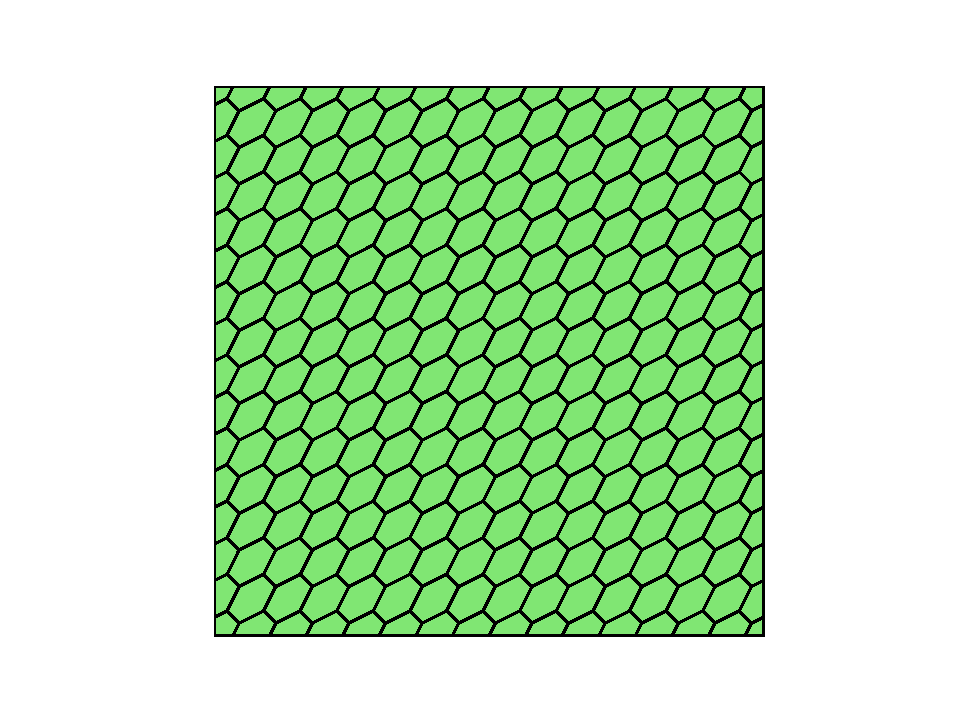
\includegraphics[width=5cm]{./figures/convex.pdf}
%\caption{Numberical result of example with $\mathcal T_0$.}
\end{minipage}%
\begin{minipage}[t]{0.49\linewidth}
\centering
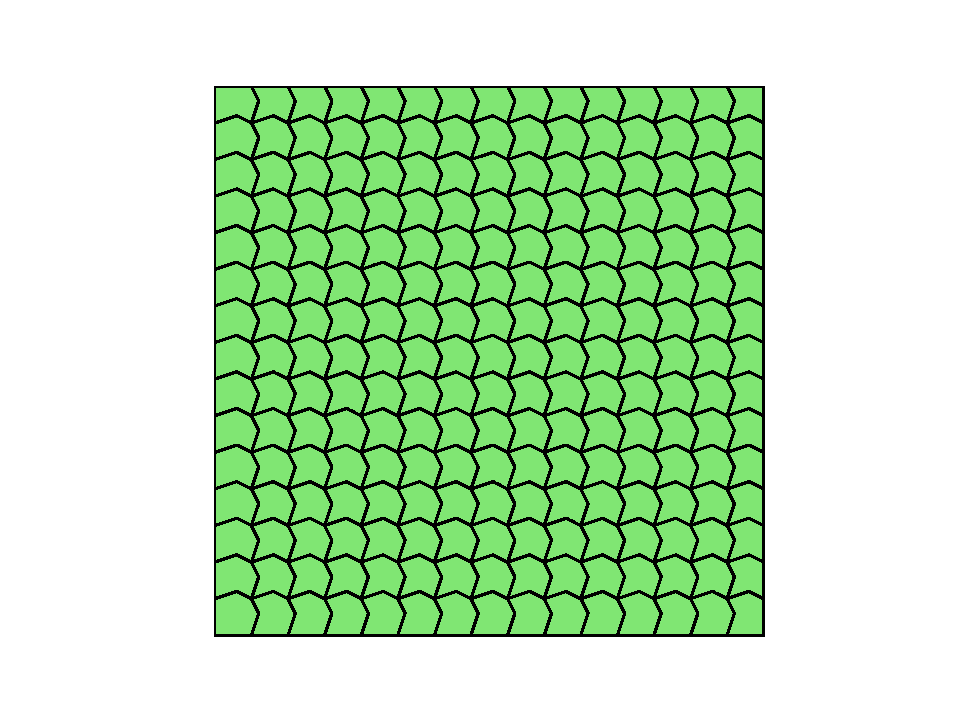
\includegraphics[width=5cm]{./figures/nonconvex.pdf}
%\caption{[Numberical result of example with $\mathcal T_1$].}
\end{minipage}%
\centering
\caption{Convex polygon mesh $\mathcal T_0$(left) and non-convex polygon mesh 
$\mathcal T_1$(right).}
\label{fig:mesh}
\end{figure}




\section{Numerical examples}\label{sec:numericalexamps}
In this section, we will numerically verify the convergence of the nonconforming virtual element method \eqref{eq:vem} and the conforming
virtual element method \eqref{eq:cfmvem}.
All of the numerical examples are implemented by using the FEALPy package \cite{fealpy}

% \begin{example}\label{ex}
Consider the second order elliptic problem \eqref{eq:ellipitc2ndproblem} with $\alpha = 2$
on rectangular domain $\Omega = (0, 1)\times(0, 1)$. 
The exact solution and source term are given by
$$
u = \sin(\pi x)\sin(\pi y), \quad f = (2\pi^2+2)\sin(\pi x)\sin(\pi y).
$$
% \end{example}

The rectangular domain $\Omega$ is partitioned by the convex polygon mesh
$\mathcal T_0$ and non-convex polygon mesh $\mathcal T_1$, respectively, 
In both virtual element methods \eqref{eq:vem} and \eqref{eq:cfmvem}, we choose $k = 1, 2, 5$.
The numerical results of the nonconforming virtual element method \eqref{eq:vem} on meshes $\mathcal T_0$ and $\mathcal T_1$ mesh are shown in Figure \ref{fig:rate1}. We can see that $\|u - Q_h u_h\|_0=O(h^{k+1})$ and $\|\nabla u - Q_{h, k-1}^{\div}\nabla_h u_h\|_0=O(h^{k})$, which coincide with Theorem~\ref{thm:errorestimateH1}.
And the numerical results of the conforming virtual element method \eqref{eq:vem} are presented in Figure \ref{fig:rate2}. Again $\|u - Q_h u_h\|_0=O(h^{k+1})$ and $\|\nabla u - Q_{h, k}^{\div}\nabla u_h\|_0=O(h^{k})$, which confirm the
theoretical convergence rate in Theorem~\ref{thm:errorestimateH1}.
\begin{figure}[htbp]
\centering
\begin{minipage}[t]{0.49\linewidth}
\centering
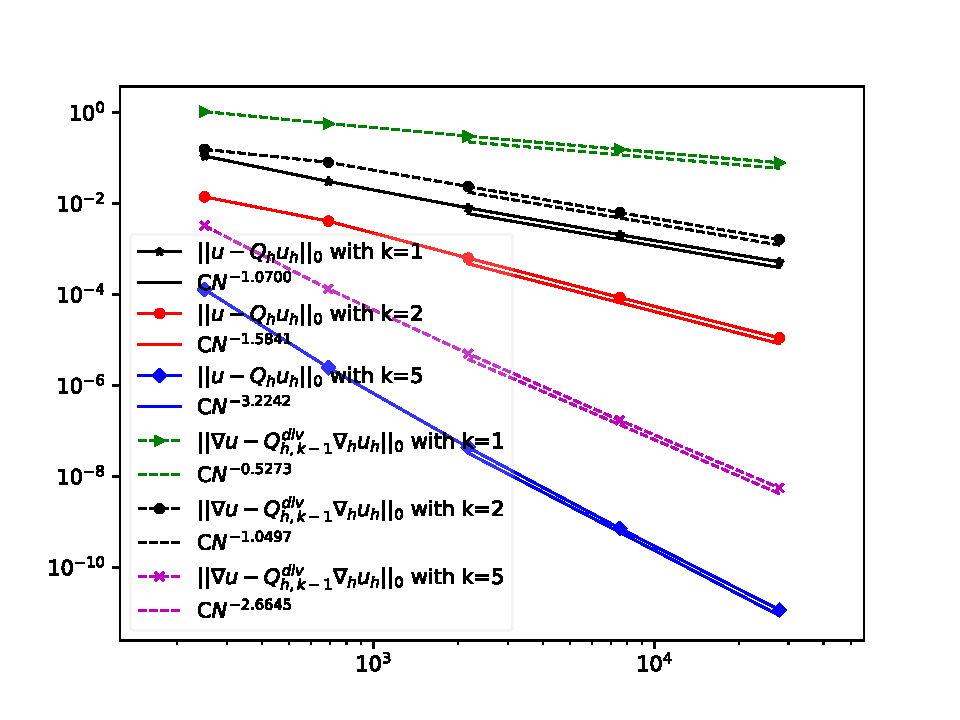
\includegraphics[width=6cm]{./figures/ncvem_convex.pdf}
%\caption{Numberical result of example with $\mathcal T_0$.}
\end{minipage}%
\begin{minipage}[t]{0.49\linewidth}
\centering
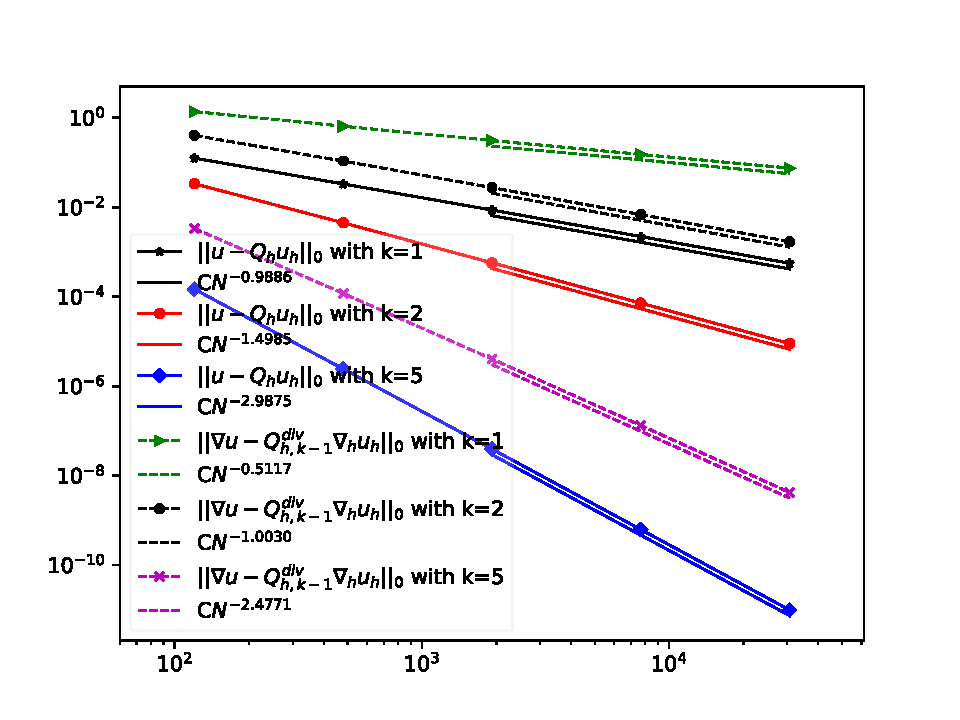
\includegraphics[width=6cm]{./figures/ncvem_nonconvex.pdf}
%\caption{[Numberical result of example with $\mathcal T_1$].}
\end{minipage}%
\centering
\caption{Errors $\|u - Q_h u_h\|_0$ and $\|\nabla u - Q_{h, k-1}^{\div}\nabla_h u_h\|_0$ 
of nonconforming virtual element method \eqref{eq:vem} on 
$\mathcal T_0$(left) and $\mathcal T_1$(right) with $k=1, 2, 5$.}
\label{fig:rate1}
\end{figure}

\begin{figure}[htbp]
\centering
\begin{minipage}[t]{0.49\linewidth}
\centering
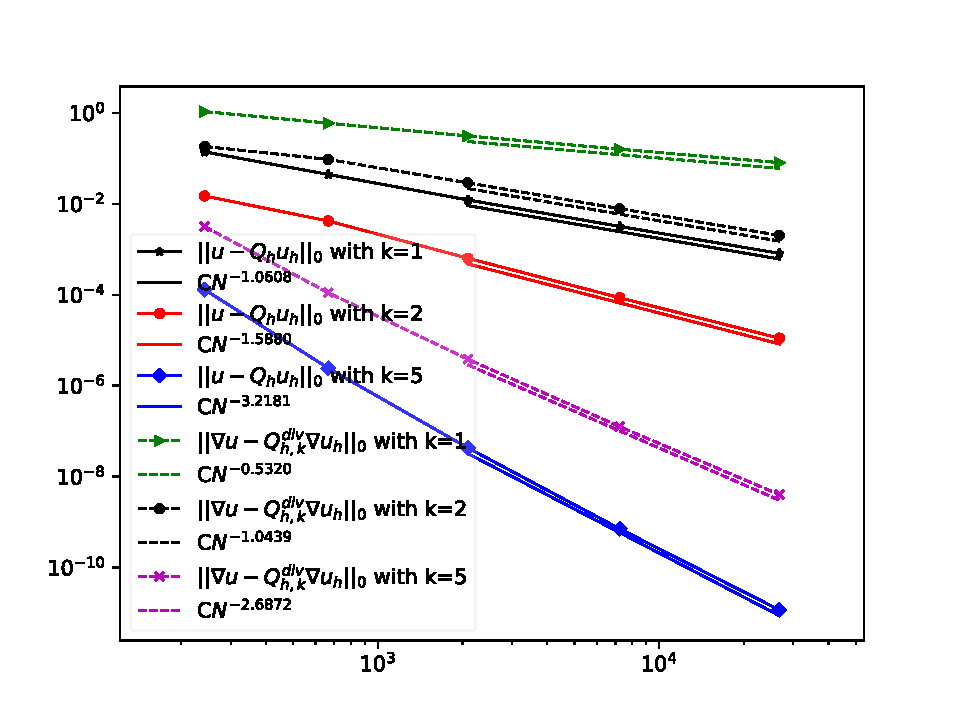
\includegraphics[width=6cm]{./figures/cvem_convex.pdf}
%\caption{Numberical result of example with $\mathcal T_0$.}
\end{minipage}%
\begin{minipage}[t]{0.49\linewidth}
\centering
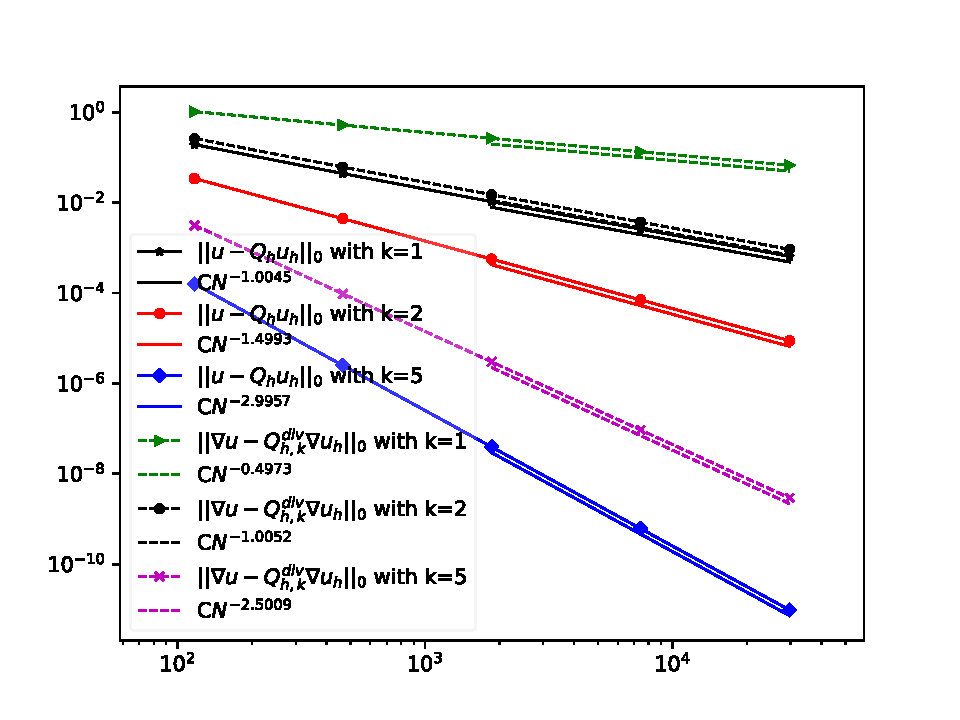
\includegraphics[width=6cm]{./figures/cvem_nonconvex.pdf}
%\caption{[Numberical result of example with $\mathcal T_1$].}
\end{minipage}%
\centering
\caption{Errors $\|u - Q_h u_h\|_0$ and $\|\nabla u - Q_{h, k}^{\div}\nabla u_h\|_0$ 
of conforming virtual element method \eqref{eq:cfmvem} on $\mathcal T_0$(left) and 
$\mathcal T_1$(right) with $k=1, 2, 5$.}
\label{fig:rate2}
\end{figure}



\bibliographystyle{abbrv}
\bibliography{./paper}
\end{document}

